\chapter{Modelagem do sistema}

A modelagem do sistema representa uma etapa fundamental no processo de desenvolvimento de \textit{software}, pois permite estruturar os requisitos, identificar restrições e representar de forma clara as responsabilidades, interações e funcionalidades esperadas da solução. Essa etapa assume especial relevância em razão da integração com dados financeiros sensíveis, da utilização de serviços externos, da comunicação por serviços de mensageria e dos requisitos relacionados à segurança, privacidade e conformidade com a Lei Geral de Proteção de Dados (LGPD).

O EIGAM é uma solução de assistência financeira inteligente, preditiva e conversacional, integrada ao ecossistema de \textit{Open Finance} e capaz de interagir com os usuários por meio de diferentes serviços de mensageria. O \textit{WhatsApp} é o principal canal de comunicação, e o \textit{Telegram} e a conversa no painel \textit{web} do titular funcionam como canais adicionais, o que demonstra que o núcleo funcional está desacoplado do provedor de mensageria.

Neste capítulo são apresentadas a fronteira sistêmica, as restrições da solução, a arquitetura da camada de inteligência artificial, os requisitos funcionais e não funcionais, os diagramas de casos de uso e suas respectivas descrições. Esses elementos delimitam o escopo do sistema, estabelecem as responsabilidades dos componentes internos e dos serviços externos envolvidos em seu funcionamento e explicitam como os mecanismos conversacionais e preditivos são distribuídos entre os serviços da aplicação.

\section{Fronteira sistêmica}

A Figura \ref{fig:fronteira} apresenta a fronteira sistêmica do EIGAM, evidenciando a separação entre os componentes pertencentes à solução e os serviços externos necessários ao seu funcionamento. Essa representação permite identificar as responsabilidades internas da aplicação, bem como os pontos de integração com sistemas de terceiros.

Externamente, a solução se comunica com seis grupos de serviços. O primeiro corresponde aos serviços de mensageria: as APIs oficiais do \textit{WhatsApp} e do \textit{Telegram}. O acesso a esses canais é intermediado por adaptadores, de modo que novos canais possam ser incorporados sem alterar o núcleo funcional da solução. O segundo é o agregador de dados de \textit{Open Finance}, por meio do qual, mediante consentimento do titular, a solução acessa e sincroniza as informações financeiras das instituições vinculadas. O terceiro corresponde aos serviços de inteligência artificial: o provedor do modelo de linguagem, utilizado no planejamento das consultas, na redação das respostas e na transcrição de áudio, e o provedor do modelo de juízo tipado que apoia os \textit{guardrails}. O quarto é o provedor de pagamentos, responsável pelas assinaturas do plano Pro. O quinto é o serviço de borda, que protege o perímetro, publica os painéis por um túnel e autentica a equipe de operação. O sexto são os assistentes de inteligência artificial do próprio titular que, mediante autorização OAuth concedida pelo titular, leem dados da solução pelo servidor MCP.

Internamente, a arquitetura separa as responsabilidades de entrada, conversa, finanças, comunicação e dados. O \textit{API Gateway} recebe os \textit{webhooks} externos; o \textit{Chat Service}, o \textit{AI Service} e o \textit{Identity Service} conduzem a conversa, a leitura da frase e a identidade do titular; o \textit{Finance Service} e o \textit{Analytics Service} processam os dados financeiros e as projeções; o \textit{Notification Service}, o \textit{Render Service} e o \textit{Outbound Worker} cuidam dos avisos, das imagens e do envio das mensagens; o \textit{Billing Service} e o \textit{Audit Service} tratam da cobrança e da auditoria. Os painéis do titular e de operação e o \textit{MCP Service}, servidor somente de leitura para os assistentes externos, completam a fronteira como interfaces expostas.

O armazenamento é distribuído de acordo com as características de cada tipo de dado. O PostgreSQL guarda as informações estruturadas e relacionais, o MongoDB atende os dados de natureza documental, o Redis gerencia sessões, estado de conversa, \textit{cache} e filas, e um \textit{broker} compatível com a API do Kafka atua como barramento de eventos entre os serviços.

Dessa forma, a fronteira sistêmica evidencia que as regras de negócio e os mecanismos de inteligência financeira permanecem independentes dos provedores externos utilizados. Essa característica permitiu que o \textit{WhatsApp} fosse o canal principal sem constituir uma dependência estrutural da solução.

\begin{figure}[H]
    \centering
    \caption{Fronteira sistêmica da solução}
    \label{fig:fronteira}
    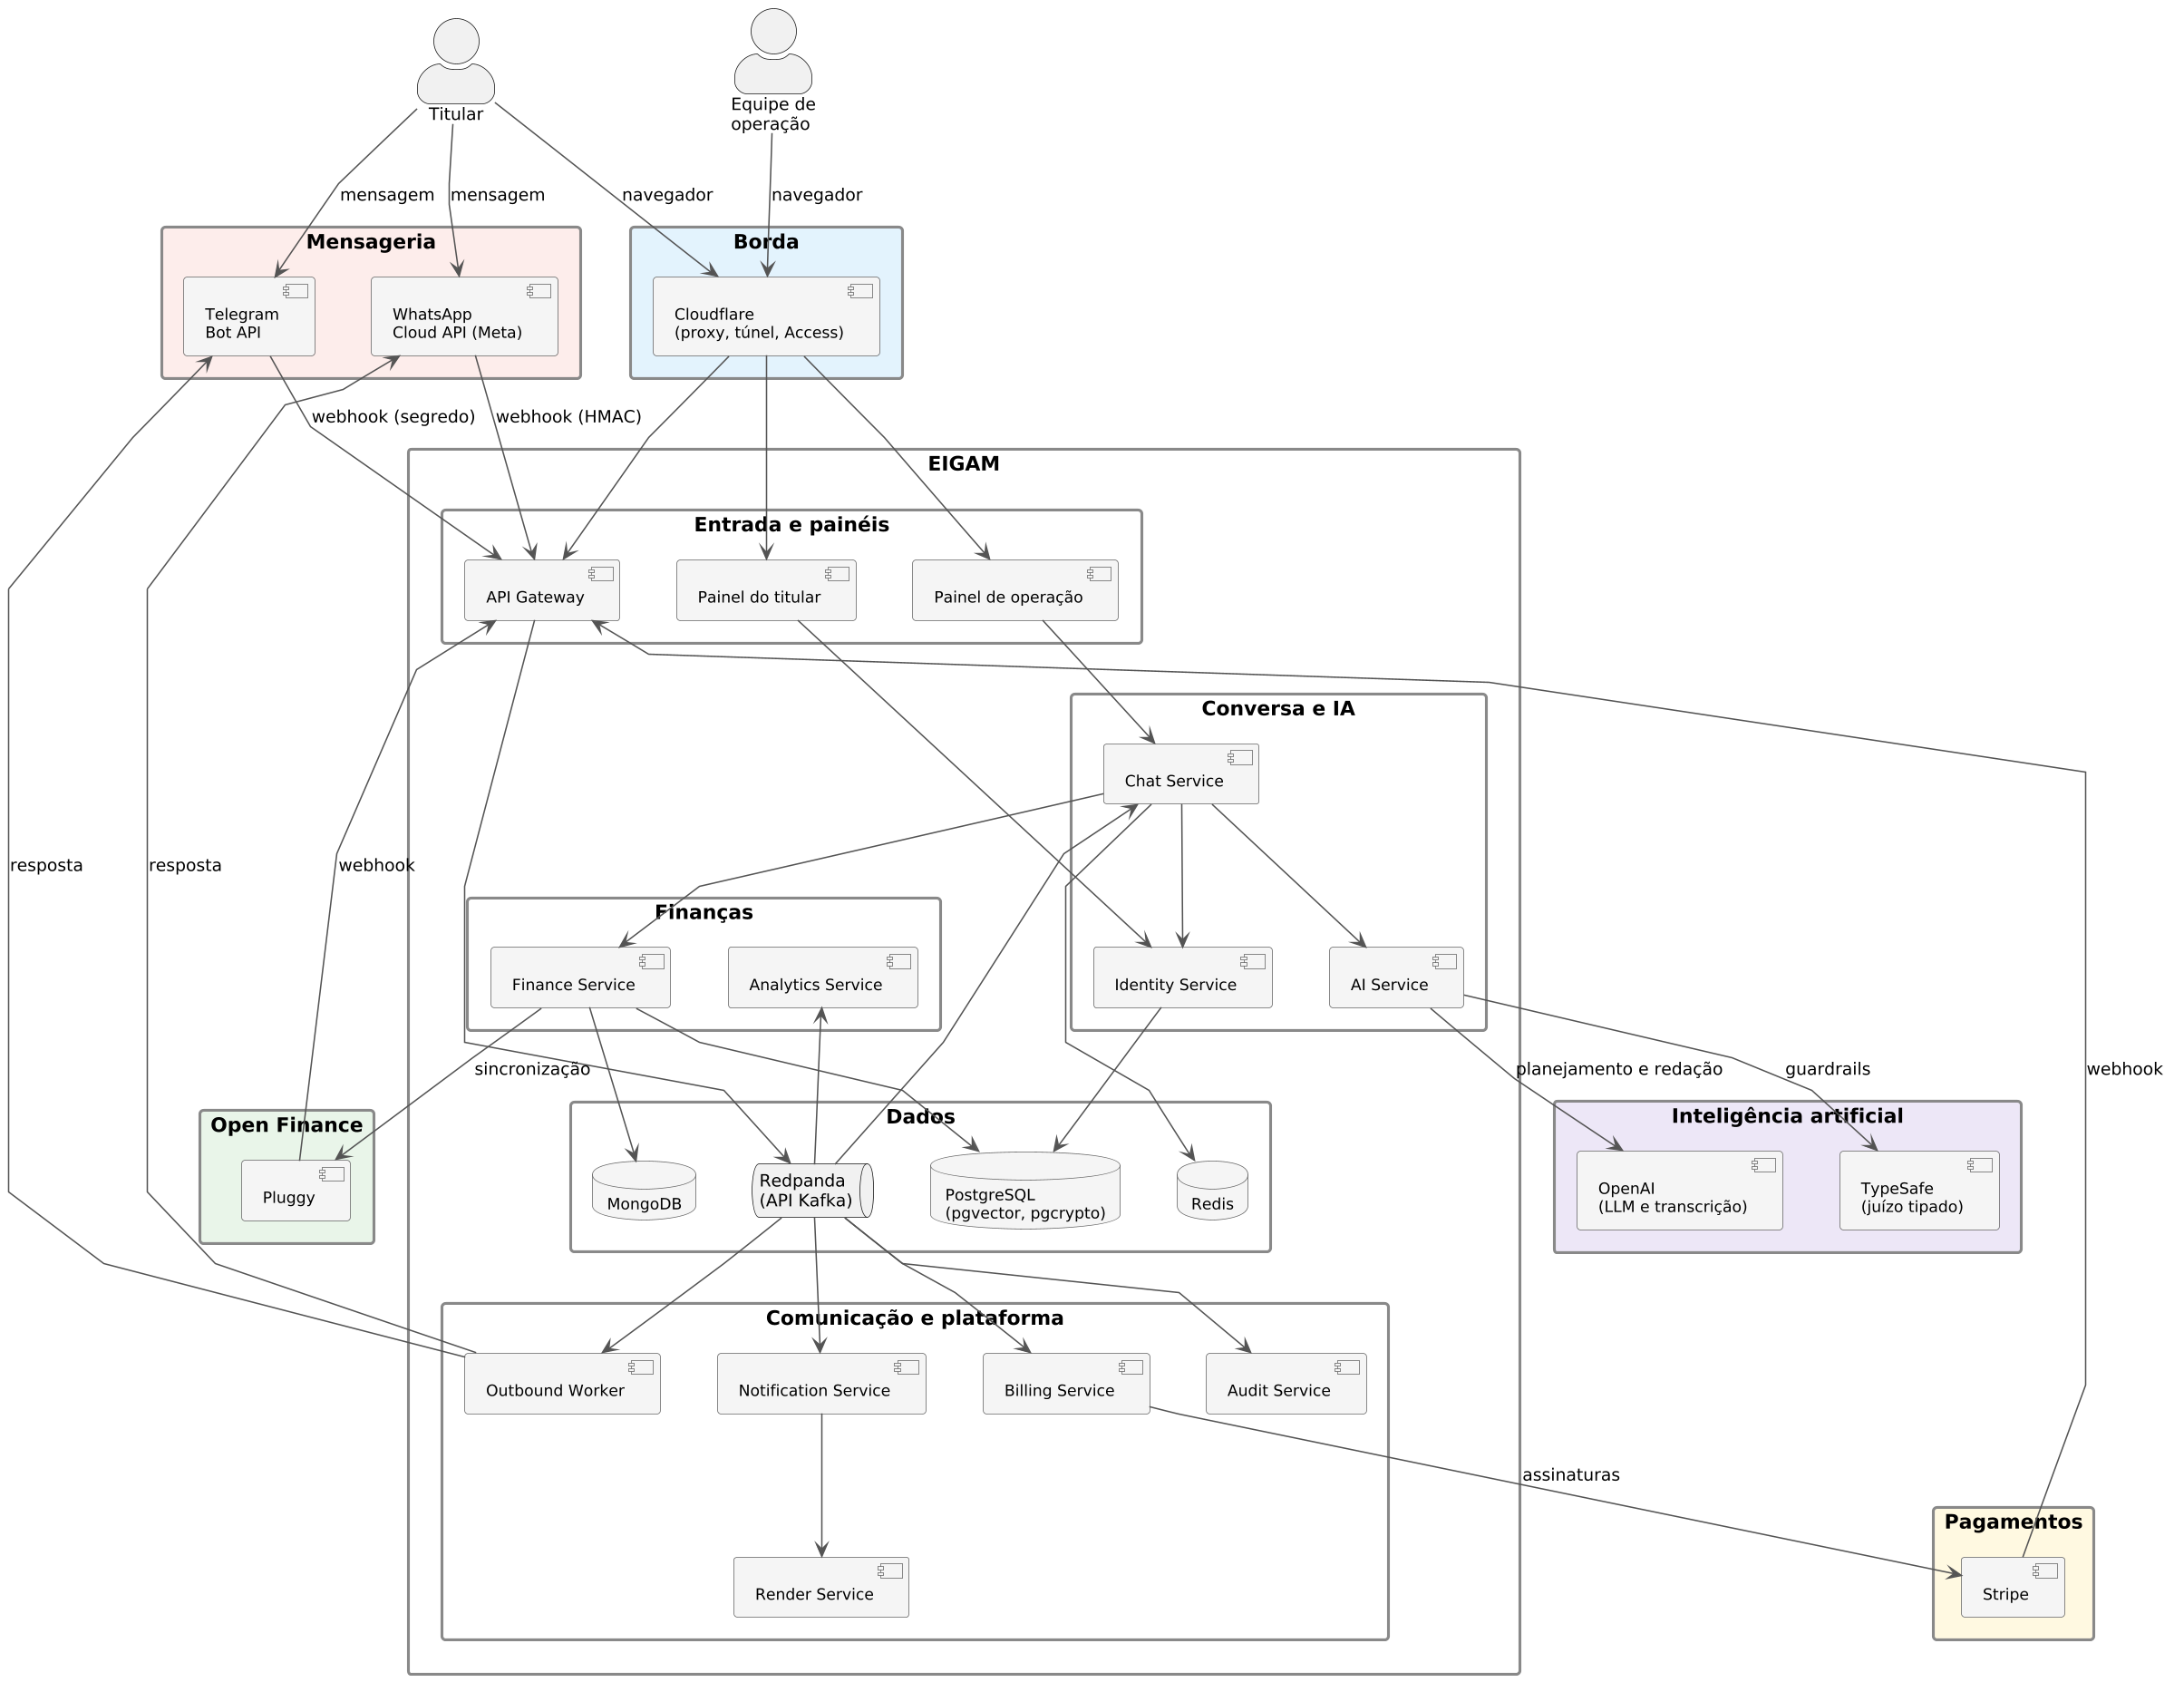
\includegraphics[width=\textwidth]{images/fronteira.png}
    \authorssource
\end{figure}

\section{Lista de restrições}

Durante a definição e a modelagem do EIGAM, foram identificadas restrições que condicionam seu funcionamento, sua arquitetura e sua capacidade de integração. Por se tratar de uma solução que depende de serviços externos, do compartilhamento autorizado de dados financeiros, de serviços de mensageria e de mecanismos de inteligência artificial, parte dessas limitações decorre de fatores que não estão sob controle direto da aplicação.

Além disso, o tratamento de dados pessoais e informações financeiras exige a observância de requisitos regulatórios e de segurança, enquanto a adoção de uma arquitetura multicanal impõe a necessidade de considerar diferenças técnicas entre os provedores de mensageria. As principais restrições identificadas são apresentadas no Quadro \ref{frame:restricoes}.

{\small
\begin{longtable}{|L{2.3cm}|L{4.0cm}|L{8.2cm}|}
\caption{Lista de Restrições} \label{frame:restricoes} \\
\continuesmark

\hline
\textbf{Origem} & \textbf{Restrição} & \textbf{Descrição} \\ \hline
\endfirsthead

\hline
\textbf{Origem} & \textbf{Restrição} & \textbf{Descrição} \\ \hline
\endhead

\endfoot
\sourcerow{3} \\
\endlastfoot

Externa &
Integração com o \textit{Open Finance} &
O acesso às informações financeiras depende da disponibilidade e das condições de funcionamento dos serviços utilizados para integração com o ecossistema de \textit{Open Finance}. No projeto, essa comunicação é intermediada por um agregador de dados, cuja indisponibilidade ou alteração em suas APIs pode afetar operações de vinculação e sincronização de dados.
\\ \hline

Externa &
Dependência de serviços de mensageria &
A comunicação com o usuário depende de APIs e serviços fornecidos por serviços externos de mensageria. O \textit{WhatsApp} é o canal principal, e alterações em políticas, preços, limites de utilização ou disponibilidade do provedor podem afetar o funcionamento desse canal.
\\ \hline

Técnica &
Interoperabilidade entre canais de mensageria &
Os serviços de mensageria possuem diferentes formatos de mensagens, recursos interativos, limites e mecanismos de autenticação. Dessa forma, a integração de novos canais deve respeitar uma interface padronizada de comunicação com o núcleo do EIGAM e adaptar as funcionalidades às capacidades disponíveis em cada canal.
\\ \hline

Técnica &
Limitações dos canais conversacionais &
Determinados recursos visuais ou interativos disponíveis em aplicações \textit{web} podem não estar presentes em todos os serviços de mensageria. A apresentação das informações deve, portanto, considerar os recursos suportados pelo canal utilizado sem comprometer o acesso às funcionalidades essenciais da solução.
\\ \hline

Regulatória &
Consentimento para acesso aos dados financeiros &
O acesso e a sincronização das informações compartilhadas por meio do \textit{Open Finance} dependem da existência de consentimento válido do titular. A revogação ou expiração desse consentimento impede novas sincronizações dos dados associados à respectiva instituição.
\\ \hline

Regulatória &
Conformidade com a LGPD &
O tratamento de dados pessoais deve observar os princípios, direitos e obrigações previstos na Lei Geral de Proteção de Dados, incluindo finalidade, necessidade, transparência, segurança e atendimento às solicitações do titular.
\\ \hline

Técnica &
Proteção das informações financeiras &
Por processar dados pessoais e informações financeiras de caráter confidencial, o sistema deve restringir sua exposição e adotar mecanismos de autenticação, autorização, controle de acesso, proteção das sessões e registro de operações relevantes.
\\ \hline

Técnica &
Disponibilidade e qualidade dos dados financeiros &
As análises realizadas pelo EIGAM dependem da disponibilidade, atualização e qualidade das informações recebidas das instituições financeiras. Dados incompletos, atrasados ou períodos históricos insuficientes podem limitar a precisão de determinadas análises, projeções e recomendações.
\\ \hline

Técnica &
Limitações dos modelos de inteligência artificial &
Os mecanismos de inteligência artificial utilizados possuem natureza probabilística e podem produzir respostas incompletas ou inadequadas. Dessa forma, o sistema deve limitar seu uso aos contextos previstos, utilizar dados financeiros validados como fonte de informação e adotar mecanismos que reduzam o risco de geração de interpretações incorretas.
\\ \hline

Externa &
Dependência de serviços terceirizados &
Partes da solução dependem de serviços externos para inteligência artificial, integração financeira, mensageria, hospedagem, monitoramento e demais recursos. Alterações de disponibilidade, limites de uso, preços ou interfaces desses fornecedores podem impactar a operação da solução.
\\ \hline

Infraestrutura &
Disponibilidade da infraestrutura em nuvem &
A solução depende de infraestrutura computacional disponível para processamento, armazenamento e execução contínua dos serviços. Falhas ou indisponibilidade do provedor de infraestrutura podem comprometer temporariamente funcionalidades da aplicação.
\\ \hline

Infraestrutura &
Disponibilidade de conexão com a \textit{internet} &
A comunicação entre o usuário, os serviços de mensageria, os serviços do EIGAM e os provedores externos depende de conectividade com a \textit{internet}. A indisponibilidade da conexão pode impedir ou atrasar consultas, sincronizações e notificações.
\\ \hline

\end{longtable}
}

\section{Arquitetura da camada de inteligência artificial}

A inteligência artificial constitui uma camada transversal da arquitetura do EIGAM, e não um serviço isolado responsável por todas as decisões da aplicação. As responsabilidades relacionadas à leitura da linguagem natural, à recuperação de contexto, à análise preditiva, à detecção de comportamentos atípicos e à comunicação proativa são distribuídas entre os serviços que possuem o contexto necessário para executá-las. Essa organização reduz o acoplamento, facilita a evolução independente dos mecanismos analíticos e evita que o modelo de linguagem seja utilizado como fonte primária de verdade para dados financeiros.

Os valores monetários, saldos, transações, agregações e resultados numéricos utilizados nas respostas são obtidos a partir de dados estruturados ou de cálculos executados pelos serviços internos. O modelo de linguagem é empregado para ler a frase do usuário, escolher as consultas necessárias e apresentar os resultados em linguagem natural. Decisões que exigem comportamento determinístico, como autenticação, mascaramento de valores, controle de acesso e execução de comandos relacionados aos direitos do titular, permanecem sob responsabilidade da aplicação.

\subsection{Distribuição das Responsabilidades de Inteligência Artificial}

A camada cognitiva do EIGAM é distribuída entre o \textit{AI Service}, o \textit{Chat Service}, o \textit{Finance Service}, o \textit{Analytics Service} e o \textit{Notification Service}. Cada serviço utiliza técnicas de inteligência artificial ou de estatística apenas nas atividades compatíveis com sua responsabilidade de domínio, conforme apresentado no Quadro \ref{frame:ia_responsabilidades}.

{\small
\begin{longtable}{|L{3.3cm}|L{11.0cm}|}
\caption{Distribuição das responsabilidades de inteligência artificial}
\label{frame:ia_responsabilidades} \\
\continuesmark
\hline
\textbf{Serviço} & \textbf{Responsabilidades relacionadas à IA} \\ \hline
\endfirsthead
\hline
\textbf{Serviço} & \textbf{Responsabilidades relacionadas à IA} \\ \hline
\endhead
\endfoot
\sourcerow{2} \\
\endlastfoot

\textit{AI Service} &
Planejador que lê a frase do titular e escolhe as consultas financeiras, redação da resposta, \textit{guardrails} de saída, leitura das respostas do cadastro, base de conhecimento sobre o produto e transcrição de notas de voz.
\\ \hline

\textit{Chat Service} &
Regras determinísticas do turno, validação e execução do plano produzido pelo modelo, cálculo dos valores em centavos e mascaramento condicional antes do envio da resposta.
\\ \hline

\textit{Finance Service} &
Tradução da categoria atribuída pelo agregador para a taxonomia do EIGAM, pareamento de lançamentos, detecção de recorrências, cálculo do gasto canônico e da posição de caixa, simulação de compra e geração dos sinais financeiros: limites de gasto, risco de estouro, cobranças duplicadas, transações atípicas e aumento de gasto por categoria.
\\ \hline

\textit{Analytics Service} &
Projeção do gasto até o fim do mês, estimativa do gasto dos meses seguintes e composição do saldo livre do fim do mês, com os métodos avaliados por teste retrospectivo em um registro de previsões, candidatos em sombra e abstenção quando nenhum método atinge o critério de aprovação.
\\ \hline

\textit{Notification Service} &
Decisão de quando avisar: preferências do titular, janela de horário, agrupamento, deduplicação e descarte de sinais que deixaram de valer. As regras que determinam se um aviso deve ser enviado não dependem do modelo de linguagem.
\\ \hline

\end{longtable}
}

Essa distribuição permite que o \textit{AI Service} concentre a interpretação da linguagem, que o \textit{Finance Service} e o \textit{Analytics Service} permaneçam responsáveis pelos cálculos e análises sobre os dados financeiros e que o \textit{Notification Service} trate a comunicação proativa. Assim, uma resposta conversacional utiliza resultados produzidos por diferentes serviços sem transferir ao modelo de linguagem a responsabilidade por calcular ou inferir valores financeiros que podem ser obtidos de maneira determinística.

\subsection{Leitura da Frase e Planejamento das Consultas}

A leitura da mensagem do titular ocorre em camadas. Antes de qualquer modelo, o \textit{Chat Service} verifica, por expressões regulares, os comandos relacionados aos direitos do titular, como consulta, exportação, revogação e exclusão de dados. Dessa forma, a execução de operações com impacto sobre os dados pessoais não depende de uma classificação probabilística. Em seguida, regras determinísticas tratam o cadastro, a troca de PIN, a conexão e a remoção de bancos, as metas, os investimentos, os empréstimos, as recorrências, a assinatura e a desconexão de assistentes externos.

As demais frases seguem para o planejador do \textit{AI Service}, que utiliza chamada de funções (\textit{function calling}) com um contrato versionado de sete funções: consulta de dados financeiros, faturas de cartão, saldos, instituições conectadas, atualização dos dados, pedido de esclarecimento e indicação de que a frase não é financeira. O modelo apenas escolhe as funções e os argumentos, como período, instituição, categoria, estabelecimento, forma de pagamento e agrupamento, e nunca responde diretamente ao titular nessa etapa. O resultado pode ser a execução das consultas, uma pergunta de esclarecimento com até três botões, uma resposta sem consulta, por exemplo para uma saudação, ou a indisponibilidade da leitura.

O \textit{Chat Service} revalida o plano com os mesmos esquemas utilizados pelos demais serviços e vincula o identificador do titular, que nunca é argumento do modelo. O planejador tem até 4,5 segundos, com uma segunda tentativa, e o \textit{Chat Service} desiste em 4,7 segundos. Nesse caso, a resposta é uma recusa sem número, e não uma estimativa.

A qualidade da leitura é medida pelo Macro-F1 do motivo devolvido pelo planejador, com mínimo de 0,88.

\subsection{Recuperação de Contexto}

O contexto fornecido ao modelo na redação da resposta tem três origens. A primeira são os fatos financeiros consultados no turno, enviados como dados estruturados e tratados como a única fonte autorizada de valores. Para as consultas mais frequentes, o servidor monta as linhas com os números exatos, e o modelo escreve apenas a abertura, a leitura e a oferta do próximo passo. A segunda é o histórico recente da conversa, que permite responder a perguntas de continuação, como ``e no mês passado?''. A terceira é uma base de conhecimento sobre o produto, com textos escritos pela equipe sobre planos, segurança, \textit{Open Finance} e direitos do titular, recuperados por palavras-chave.

Os dados recuperados são tratados como contexto da resposta, e não como instruções. Descrições de transações, nomes de metas e de estabelecimentos entram no prompt neutralizados, sem quebras de linha, delimitadores ou contatos, o que reduz a superfície para tentativas de manipulação.

\subsection{Análise Preditiva e Detecção de Anomalias}

A camada preditiva do EIGAM não depende de modelos generativos. Para tarefas numéricas e de séries temporais, são utilizados métodos estatísticos, e a geração textual permanece separada do cálculo dos resultados.

A projeção estima o gasto até o fim do mês corrente, no total ou por categoria. O modelo servido é o ritmo robusto, que estende aos dias restantes apenas o gasto típico, e os demais candidatos continuam calculados em sombra em um registro de previsões, fechado mensalmente contra o valor real.

Duas estimativas complementares integram a mesma camada. O saldo livre do fim do mês opera em regime de caixa: parte do saldo disponível das contas correntes, desconta faturas a vencer, recorrentes em conta e agendamentos, e estima o movimento líquido restante pela mediana dos seis meses anteriores, cuja amplitude define a faixa da resposta; a resposta recusa com motivo declarado quando falta histórico ou quando alguma conexão está desatualizada. A simulação de compra aplica uma compra hipotética, à vista ou parcelada e com o calendário de fechamento do cartão, sobre a estimativa do fim do mês, a folga das metas e os compromissos dos doze meses seguintes, sem emitir juízo sobre a compra.

A detecção de transações atípicas compara o valor de cada transação recente com o histórico de gastos da mesma categoria por meio de um escore-z robusto, calculado sobre o logaritmo do valor com a mediana e o desvio absoluto mediano, menos sensíveis a valores extremos do que a média e o desvio-padrão. O sinal é emitido a partir de 3,5, exige pelo menos dez transações e noventa dias de histórico, e recebe confiança alta a partir de 5 com vinte transações. Além disso, o \textit{Finance Service} detecta possíveis cobranças duplicadas, aumento de gasto em uma categoria em relação ao padrão do titular e a travessia de 80\% e de 100\% dos limites de gasto definidos nas metas, bem como o risco de ultrapassá-los até o fim do período.

Os limiares são parâmetros configuráveis. Sempre que não há histórico suficiente para determinada análise, o sistema evita apresentar conclusões e informa ao usuário que são necessários mais dados.

\subsection{Mecanismos de Controle e Confiabilidade}

Por operar em um domínio que envolve informações financeiras, o EIGAM adota mecanismos de controle adicionais sobre as respostas produzidas pelos modelos de linguagem. Esses controles, também denominados \textit{guardrails}, atuam antes da entrega da resposta ao usuário e reduzem os riscos relacionados à exposição indevida de valores, à geração de informações sem origem verificável, às solicitações fora do escopo e às tentativas de manipulação das instruções do sistema.

O Quadro \ref{frame:guardrails_ia} apresenta os controles implementados na camada conversacional.

{\small
\begin{longtable}{|L{3.7cm}|L{5.2cm}|L{5.4cm}|}
\caption{Mecanismos de controle da camada conversacional}
\label{frame:guardrails_ia} \\
\continuesmark
\hline
\textbf{Controle} & \textbf{Verificação} & \textbf{Ação} \\ \hline
\endfirsthead
\hline
\textbf{Controle} & \textbf{Verificação} & \textbf{Ação} \\ \hline
\endhead
\endfoot
\sourcerow{3} \\
\endlastfoot

Exposição de valores não autorizados &
Verifica se o titular possui token de privilégio válido para exibição de valores monetários. &
Aplica mascaramento determinístico por expressão regular no servidor, depois do modelo, e indica que o PIN libera os valores.
\\ \hline

Valores sem origem verificável &
Nas respostas tipadas, compara as frases do modelo com os fatos consultados no turno. &
O servidor monta as linhas com os valores exatos e descarta a frase do modelo que traga valor fora dos fatos.
\\ \hline

Conselho regulado &
Identifica recomendação de investimento, ações, criptoativos ou tributos, por expressão regular e por um modelo de juízo tipado. &
Substitui a resposta por um texto fixo; a pergunta de alocação explícita é recusada antes de chegar ao modelo.
\\ \hline

Pedido de credencial &
Identifica resposta que solicite senha bancária, CPF, código ou dados de cartão. &
Substitui a resposta por um texto fixo, sem depender do modelo.
\\ \hline

Conteúdo fora do escopo &
O planejador indica que a frase não pertence ao escopo do produto. &
Recusa por \textit{template}, sem chamar o modelo de redação.
\\ \hline

Exposição de instruções internas &
Busca trechos do prompt ou marcadores internos na resposta. &
Substitui a resposta por um texto fixo.
\\ \hline

Tentativas de \textit{prompt injection} &
Identifica, na mensagem do usuário, padrões destinados a substituir, ignorar ou revelar instruções internas, por expressão regular e por modelo de juízo. &
Desconsidera a instrução maliciosa e responde com texto fixo.
\\ \hline

Contato não informado pelo titular &
Busca \textit{links}, telefones, e-mails ou chaves Pix que o titular não escreveu. &
Descarta a resposta.
\\ \hline

Comprimento e oferta &
Verifica resposta vazia ou acima de 2.800 caracteres e oferta de próximo passo não autorizado. &
Corta a resposta, usa o \textit{template} de contingência ou troca a oferta por uma autorizada.
\\ \hline

\end{longtable}
}

O mascaramento de valores financeiros é executado de maneira determinística pela aplicação, e não pelo modelo de linguagem. Da mesma forma, o modelo não recebe autoridade para validar autenticação, alterar consentimentos, executar exclusões ou decidir quais dados podem ser apresentados. A separação entre geração textual e regras de autorização garante que falhas de interpretação do modelo não resultem diretamente em exposição indevida de informações ou execução de operações sensíveis. Com o provedor do modelo de juízo indisponível, o \textit{guardrail} de conselho falha de forma fechada: respostas que comparem produtos financeiros são recusadas em vez de liberadas.

A confiabilidade dessa camada foi avaliada por testes específicos, incluindo a leitura da frase pelo planejador, a consistência das informações numéricas, a robustez diante de entradas adversariais e o desempenho dos modelos preditivos. Os critérios e os resultados dessas medições são apresentados nos Capítulos \ref{chap:desenvolvimento} e \ref{chap:resultados}.

\section{Requisitos e diagramas}

A definição dos requisitos é uma das etapas centrais do desenvolvimento de \textit{software}, pois estabelece com precisão o que a solução deve ser capaz de realizar e sob quais condições deve operar. De acordo com Washizaki (2024), no \textit{Guide to the Software Engineering Body of Knowledge} (SWEBOK), a engenharia de requisitos integra uma das áreas de conhecimento fundamentais da engenharia de \textit{software}, sendo responsável por apoiar a identificação, documentação e comunicação das necessidades do sistema. Complementarmente, o uso de diagramas de casos de uso auxilia na representação visual das interações entre os usuários e o sistema, facilitando a compreensão do escopo e a comunicação entre os envolvidos no projeto.

\subsection{Requisitos Funcionais}

O Quadro \ref{frame:rf} apresenta os requisitos funcionais do projeto, isto é, as funcionalidades e comportamentos que o sistema deve oferecer para atender às necessidades dos usuários. Esses requisitos abrangem desde o cadastro e a vinculação de contas bancárias até a consulta de informações financeiras, a geração de análises e previsões, o envio de alertas, o gerenciamento de metas e o gerenciamento de consentimentos, refletindo os principais fluxos de interação da solução.

\begin{longtable}{|L{1.5cm}|L{3.2cm}|L{7.3cm}|L{2.1cm}|}
\caption{Requisitos Funcionais} \label{frame:rf} \\
\continuesmark
\hline
\textbf{Código} & \textbf{Requisito} & \textbf{Descrição} & \textbf{Prioridade} \\ \hline
\endfirsthead
\hline
\textbf{Código} & \textbf{Requisito} & \textbf{Descrição} & \textbf{Prioridade} \\ \hline
\endhead
\endfoot
\sourcerow{4} \\
\endlastfoot
{[RF001]} & Realizar cadastro & O usuário deve ser capaz de iniciar seu cadastro na solução por meio do WhatsApp ou de outro canal de mensageria, fornecendo as informações necessárias para criação de sua conta. & Obrigatório \\ \hline
{[RF002]} & Vincular conta ao \textit{Open Finance} & O usuário deve ser capaz de autorizar e vincular suas contas bancárias por meio do \textit{Open Finance}, permitindo o compartilhamento de dados financeiros com a solução. & Obrigatório \\ \hline
{[RF003]} & Consultar informações financeiras & O usuário deve ser capaz de consultar, por meio da conversa, informações como saldo, transações, histórico financeiro, movimentações recentes e resumos financeiros periódicos com visão consolidada de receitas, despesas e saldo. & Obrigatório \\ \hline
{[RF004]} & Gerar análises financeiras & O sistema deve ser capaz de analisar os dados financeiros do usuário e apresentar interpretações sobre gastos, receitas e comportamento financeiro. & Obrigatório \\ \hline
{[RF005]} & Gerar previsões financeiras & O sistema deve ser capaz de produzir previsões com base no histórico financeiro do usuário, indicando possíveis cenários futuros relacionados a gastos e saldo. & Obrigatório \\ \hline
{[RF006]} & Emitir alertas financeiros & O sistema deve ser capaz de enviar alertas ao usuário sobre situações relevantes, como vencimentos, gastos acima do padrão ou risco de saldo insuficiente. & Obrigatório \\ \hline
{[RF007]} & Fornecer recomendações personalizadas & O sistema deve ser capaz de gerar orientações e recomendações financeiras personalizadas com base no perfil e no histórico do usuário. & Obrigatório \\ \hline
{[RF008]} & Definir metas financeiras & O usuário deve ser capaz de cadastrar metas financeiras, como economizar determinado valor ou controlar gastos em categorias específicas. & Desejável \\ \hline
{[RF009]} & Acompanhar metas financeiras & O usuário deve ser capaz de consultar o andamento de suas metas financeiras por meio da conversa. & Desejável \\ \hline
{[RF010]} & Gerenciar consentimento & O usuário deve ser capaz de conceder, visualizar e revogar o consentimento de acesso aos seus dados financeiros compartilhados, incluindo a desvinculação de contas bancárias da solução. & Obrigatório \\ \hline
{[RF011]} & Gerenciar perfil & O usuário deve ser capaz de visualizar e atualizar suas informações cadastrais e preferências de uso da solução. & Desejável \\ \hline
{[RF012]} & Disponibilizar painel administrativo & O sistema deve fornecer uma área administrativa para acompanhamento técnico e gerenciamento geral da solução. & Desejável \\ \hline
{[RF013]} & Disponibilizar painel do titular & O usuário deve ser capaz de acessar, por um navegador, uma extensão da conversa para consultar o mês, as transações, os bancos conectados, a assinatura e a privacidade, com os mesmos controles de mascaramento da conversa. & Desejável \\ \hline
\end{longtable}

\subsection{Requisitos Não Funcionais e de Qualidade}

Além dos requisitos funcionais, a solução deve atender a requisitos não funcionais e de qualidade que assegurem seu funcionamento adequado em um contexto de alta sensibilidade de dados. Dado que a solução lida com informações financeiras e pessoais de usuários, aspectos como segurança, privacidade, confiabilidade e desempenho são tratados como prioridades estruturais. O detalhamento desses requisitos é apresentado no Quadro \ref{frame:rnf}.

\begin{longtable}{|L{1.8cm}|L{3.2cm}|L{7.0cm}|L{2.1cm}|}
\caption{Requisitos Não Funcionais e de Qualidade} \label{frame:rnf} \\
\continuesmark
\hline
\textbf{Código} & \textbf{Requisito} & \textbf{Descrição} & \textbf{Prioridade} \\ \hline
\endfirsthead
\hline
\textbf{Código} & \textbf{Requisito} & \textbf{Descrição} & \textbf{Prioridade} \\ \hline
\endhead
\endfoot
\sourcerow{4} \\
\endlastfoot
{[RNF001]} & Segurança dos dados & O sistema deve proteger os dados pessoais e financeiros do usuário contra acessos não autorizados, vazamentos e usos indevidos. & Obrigatório \\ \hline
{[RNF002]} & Privacidade das informações & O sistema deve tratar os dados do usuário em conformidade com a LGPD, garantindo consentimento, transparência e controle sobre o uso das informações. & Obrigatório \\ \hline
{[RNF003]} & Disponibilidade do sistema & O sistema deve permanecer disponível para uso na maior parte do tempo, permitindo o acesso contínuo às funcionalidades essenciais. & Obrigatório \\ \hline
{[RNF004]} & Desempenho nas respostas & O sistema deve fornecer respostas ao usuário em tempo adequado, de modo a manter a interação conversacional fluida e eficiente. & Obrigatório \\ \hline
{[RNF005]} & Usabilidade & O sistema deve apresentar interações em linguagem natural, simples, claras e de fácil compreensão, adequadas ao uso por meio de interface conversacional no WhatsApp. & Obrigatório \\ \hline
{[RNF006]} & Confiabilidade das informações & O sistema deve apresentar dados financeiros, análises e alertas de forma consistente e confiável, reduzindo o risco de interpretações incorretas. & Obrigatório \\ \hline
{[RNF007]} & Escalabilidade & O sistema deve ser capaz de suportar o aumento do número de usuários e interações sem comprometer seu funcionamento. & Desejável \\ \hline
{[RNF008]} & Integração com serviços externos & O sistema deve ser compatível com APIs e serviços externos necessários para integração com \textit{Open Finance}, WhatsApp e demais recursos utilizados. & Obrigatório \\ \hline
{[RNF009]} & Manutenibilidade & O sistema deve ser desenvolvido de forma organizada e modular, facilitando correções, ajustes e futuras evoluções. & Obrigatório \\ \hline
{[RNF010]} & Portabilidade & O sistema deve funcionar adequadamente em diferentes dispositivos que suportem o WhatsApp ou o Telegram e, no caso do painel do titular, em navegadores web de computadores e celulares. & Desejável \\ \hline
{[RNF011]} & Autenticação segura & O sistema deve utilizar mecanismos seguros de autenticação e validação de identidade para acesso às informações financeiras do usuário. & Obrigatório \\ \hline
{[RNF012]} & Auditabilidade & O sistema deve ser capaz de registrar ações relevantes e eventos importantes para fins de monitoramento, rastreabilidade e suporte. & Desejável \\ \hline
{[RNF013]} & Clareza na comunicação & O sistema deve apresentar mensagens e respostas em linguagem clara, objetiva e compreensível para o usuário final. & Obrigatório \\ \hline
{[RNF014]} & Precisão das previsões e recomendações & O sistema deve buscar manter nível adequado de precisão nas previsões e recomendações geradas com base nos dados financeiros do usuário. & Obrigatório \\ \hline
{[RNF015]} & Recuperação de falhas & O sistema deve ser capaz de lidar com falhas de integração, indisponibilidade de serviços externos ou erros de processamento sem comprometer totalmente sua operação. & Desejável \\ \hline
{[RNF016]} & Compatibilidade com o canal conversacional & O sistema deve respeitar as limitações e diretrizes de operação do \textit{WhatsApp Business}. & Obrigatório \\ \hline
{[RNF017]} & Acessibilidade textual & O sistema deve priorizar mensagens objetivas e bem estruturadas, facilitando a compreensão por diferentes perfis de usuários. & Desejável \\ \hline
{[RNF018]} & Atualização de dados & O sistema deve manter as informações financeiras do usuário sincronizadas com frequência adequada, de acordo com a disponibilidade das integrações. & Obrigatório \\ \hline
\end{longtable}

\subsection{Diagrama de Casos de Uso}

Os diagramas de caso de uso são utilizados para representar, de forma visual, as interações entre os atores externos e o sistema, evidenciando as funcionalidades oferecidas e os objetivos que podem ser alcançados por meio dessas interações (Object Management Group, 2017). Dessa forma, esses diagramas auxiliam na compreensão do escopo do sistema e na comunicação dos requisitos levantados durante o projeto.

A solução foi modelada em quatro grupos funcionais de casos de uso: acesso e consulta financeira, análise preditiva e alertas, metas financeiras e resumos periódicos, e direitos do titular conforme a LGPD (Art.\ 18). As Figuras \ref{fig:uc01}, \ref{fig:uc02}, \ref{fig:uc03} e \ref{fig:uc04} apresentam os diagramas correspondentes a cada grupo.

\begin{figure}[H]
    \centering
    \caption{Diagrama de Casos de Uso - Acesso e Consulta Financeira}
    \label{fig:uc01}
    \includegraphics[width=1\textwidth]{"images/uml/UC01 - Acesso e Consulta Financeira.png"}
    \authorssource
\end{figure}

\begin{figure}[H]
    \centering
    \caption{Diagrama de Casos de Uso - Análise Preditiva e Alertas}
    \label{fig:uc02}
    \includegraphics[width=1\textwidth]{"images/uml/UC02 - Analise Preditiva e Alertas.png"}
    \authorssource
\end{figure}

\begin{figure}[H]
    \centering
    \caption{Diagrama de Casos de Uso - Metas Financeiras e Resumos Periódicos}
    \label{fig:uc03}
    \includegraphics[width=1\textwidth]{"images/uml/UC03 - Metas Financeiras e Resumos Periodicos.png"}
    \authorssource
\end{figure}

\begin{figure}[H]
    \centering
    \caption{Diagrama de Casos de Uso - Direitos do Titular (LGPD Art.\ 18)}
    \label{fig:uc04}
    \includegraphics[width=1\textwidth]{"images/uml/UC04 - Direitos do Titular (LGPD Art. 18).png"}
    \authorssource
\end{figure}

\subsection{Descrição de Casos de Uso}

A seguir são apresentadas as descrições textuais dos casos de uso identificados nos diagramas, organizadas conforme os quatro grupos funcionais da solução.

\noindent\textbf{Grupo 1 - Acesso e Consulta Financeira}

\vspace{4pt}

Os quadros \ref{frame:uc001} a \ref{frame:uc028} descrevem os casos de uso relativos ao acesso e à consulta financeira, abrangendo o cadastro do usuário, a vinculação de contas bancárias via \textit{Open Finance}, a autenticação pelo PIN de 6 dígitos, as operações de consulta de saldo, extrato e resumo financeiro e o acesso ao painel do titular.

\vspace{4pt}

{\small
\begin{longtable}{|L{3.5cm}|L{11.0cm}|}
\caption{[UC001] Realizar cadastro pela conversa} \label{frame:uc001} \\
\continuesmark
\hline
\endfirsthead
\hline
\endhead
\endfoot
\sourcerow{2} \\
\endlastfoot
\textbf{Caso de uso} & [UC001] Realizar cadastro pela conversa \\ \hline
\textbf{Ator(es)} & Usuário \\ \hline
\textbf{Motivação} & Permitir que um novo usuário crie sua conta pela conversa no \textit{WhatsApp} ou no \textit{Telegram}, ou pelo formulário do canal, definindo suas credenciais de acesso. \\ \hline
\textbf{Fluxo Principal} &
1. O usuário envia uma mensagem inicial ao assistente;\newline
2. O sistema se apresenta e oferece o aceite dos termos de uso e da política de privacidade; antes disso, o usuário pode tirar dúvidas sobre o produto ou experimentar o assistente com dados de demonstração;\newline
3. O usuário aceita os termos e informa nome, CPF e e-mail;\newline
4. O sistema solicita a criação de um PIN de 6 dígitos;\newline
5. O usuário define e confirma o PIN;\newline
6. O sistema armazena o PIN com \textit{bcrypt} (12 \textit{salt rounds}), cifra os dados pessoais e conclui o cadastro;\newline
7. O sistema confirma o cadastro e oferece a conexão de uma conta bancária.
\\ \hline
\textbf{Fluxo Alternativo} &
a. Os PINs digitados não coincidem:\newline
\hspace*{1em}i. O sistema informa que os PINs não coincidem;\newline
\hspace*{1em}ii. O processo retorna à fase 4 do fluxo principal.\newline
b. O CPF informado é inválido:\newline
\hspace*{1em}i. O sistema informa o erro e solicita o CPF novamente.\newline
c. O usuário recusa os termos:\newline
\hspace*{1em}i. O sistema não cria a conta;\newline
\hspace*{1em}ii. O usuário continua podendo fazer perguntas sobre o produto.
\\ \hline
\end{longtable}
}

\vspace{4pt}

{\small
\begin{longtable}{|L{3.5cm}|L{11.0cm}|}
\caption{[UC002] Vincular conta ao \textit{Open Finance}} \label{frame:uc002} \\
\continuesmark
\hline
\endfirsthead
\hline
\endhead
\endfoot
\sourcerow{2} \\
\endlastfoot
\textbf{Caso de uso} & [UC002] Vincular conta ao \textit{Open Finance} \\ \hline
\textbf{Ator(es)} & Usuário, Agregador (\textit{Open Finance}) \\ \hline
\textbf{Motivação} & Permitir ao usuário autorizar o acesso a seus dados bancários via \textit{Open Finance} por meio da integração com o agregador de dados, escolhendo por quanto tempo o compartilhamento deve valer. \\ \hline
\textbf{Fluxo Principal} &
1. O usuário solicita a vinculação de conta bancária;\newline
2. O sistema solicita a escolha da instituição e do prazo do consentimento (3, 6 ou 12 meses, ou até cancelar);\newline
3. O sistema gera o link de autorização do agregador e o envia ao usuário;\newline
4. O usuário autoriza o compartilhamento no ambiente do próprio banco;\newline
5. O agregador notifica o sistema por \textit{webhook};\newline
6. O sistema registra o consentimento e envia o comprovante da conexão em imagem;\newline
7. O sistema realiza a primeira sincronização dos dados.
\\ \hline
\textbf{Fluxo Alternativo} &
a. O usuário não aceitou os termos:\newline
\hspace*{1em}i. O sistema solicita o aceite antes de gerar o link.\newline
b. O usuário não conclui a autorização no banco:\newline
\hspace*{1em}i. A vinculação não é realizada;\newline
\hspace*{1em}ii. O sistema informa que a vinculação está pendente.
\\ \hline
\end{longtable}
}

\vspace{4pt}

{\small
\begin{longtable}{|L{3.5cm}|L{11.0cm}|}
\caption{[UC003] Autenticar via PIN de 6 dígitos} \label{frame:uc003} \\
\continuesmark
\hline
\endfirsthead
\hline
\endhead
\endfoot
\sourcerow{2} \\
\endlastfoot
\textbf{Caso de uso} & [UC003] Autenticar via PIN de 6 dígitos \\ \hline
\textbf{Ator(es)} & Usuário \\ \hline
\textbf{Motivação} & Garantir a autenticação do titular antes da exibição de valores monetários, emitindo um token de privilégio (inclui [UC009]). \\ \hline
\textbf{Fluxo Principal} &
1. O sistema solicita ao usuário o PIN de 6 dígitos;\newline
2. O usuário digita o PIN;\newline
3. O sistema valida o PIN utilizando \textit{bcrypt};\newline
4. O sistema emite o token de privilégio ([UC009]);\newline
5. Os valores monetários passam a ser exibidos na conversa e no painel, e as respostas passam a poder incluir imagens.
\\ \hline
\textbf{Fluxo Alternativo} &
a. O PIN informado está incorreto:\newline
\hspace*{1em}i. O sistema notifica o usuário e solicita nova tentativa;\newline
\hspace*{1em}ii. Após 5 tentativas incorretas, o sistema bloqueia o acesso por 30 minutos.\newline
b. O usuário envia o PIN por nota de voz:\newline
\hspace*{1em}i. O áudio não é transcrito;\newline
\hspace*{1em}ii. O sistema pede que o PIN seja digitado.
\\ \hline
\end{longtable}
}

\vspace{4pt}

{\small
\begin{longtable}{|L{3.5cm}|L{11.0cm}|}
\caption{[UC004] Consultar saldo e extrato} \label{frame:uc004} \\
\continuesmark
\hline
\endfirsthead
\hline
\endhead
\endfoot
\sourcerow{2} \\
\endlastfoot
\textbf{Caso de uso} & [UC004] Consultar saldo e extrato \\ \hline
\textbf{Ator(es)} & Usuário, Agregador (\textit{Open Finance}) \\ \hline
\textbf{Motivação} & Permitir ao usuário consultar o saldo atual e o extrato de forma conversacional, com os dados da última sincronização das instituições conectadas (inclui [UC003] e [UC007]). \\ \hline
\textbf{Fluxo Principal} &
1. O usuário solicita saldo ou extrato ao assistente;\newline
2. O sistema interpreta a pergunta e consulta os dados sincronizados;\newline
3. O sistema verifica o token de privilégio;\newline
4. O sistema gera uma resposta em linguagem natural ([UC007]);\newline
5. O sistema apresenta o saldo e/ou o extrato ao usuário.
\\ \hline
\textbf{Fluxo Alternativo} &
a. O token de privilégio não está ativo:\newline
\hspace*{1em}i. O sistema exibe os valores mascarados (R\$ •••••);\newline
\hspace*{1em}ii. O sistema informa que o PIN libera os valores ([UC003]).\newline
b. A sincronização com o agregador está atrasada ou indisponível:\newline
\hspace*{1em}i. O sistema informa a data da última atualização;\newline
\hspace*{1em}ii. O sistema apresenta os últimos dados sincronizados.
\\ \hline
\end{longtable}
}

\vspace{4pt}

{\small
\begin{longtable}{|L{3.5cm}|L{11.0cm}|}
\caption{[UC005] Consultar histórico de transações} \label{frame:uc005} \\
\continuesmark
\hline
\endfirsthead
\hline
\endhead
\endfoot
\sourcerow{2} \\
\endlastfoot
\textbf{Caso de uso} & [UC005] Consultar histórico de transações \\ \hline
\textbf{Ator(es)} & Usuário, Agregador (\textit{Open Finance}) \\ \hline
\textbf{Motivação} & Permitir ao usuário consultar o histórico de transações por período, banco, categoria, estabelecimento ou forma de pagamento (inclui [UC003] e [UC007]). \\ \hline
\textbf{Fluxo Principal} &
1. O usuário solicita o histórico de transações ao assistente;\newline
2. O sistema identifica o recorte pedido e consulta as transações sincronizadas;\newline
3. O sistema verifica o token de privilégio;\newline
4. O sistema gera uma resposta em linguagem natural ([UC007]);\newline
5. O sistema apresenta o histórico ao usuário.
\\ \hline
\textbf{Fluxo Alternativo} &
a. O token de privilégio não está ativo:\newline
\hspace*{1em}i. O sistema exibe os valores mascarados (R\$ •••••);\newline
\hspace*{1em}ii. O sistema informa que o PIN libera os valores ([UC003]).\newline
b. O banco citado não está conectado:\newline
\hspace*{1em}i. O sistema informa que o banco não está conectado e oferece a conexão.
\\ \hline
\end{longtable}
}

\vspace{4pt}

{\small
\begin{longtable}{|L{3.5cm}|L{11.0cm}|}
\caption{[UC006] Consultar resumo financeiro} \label{frame:uc006} \\
\continuesmark
\hline
\endfirsthead
\hline
\endhead
\endfoot
\sourcerow{2} \\
\endlastfoot
\textbf{Caso de uso} & [UC006] Consultar resumo financeiro \\ \hline
\textbf{Ator(es)} & Usuário, Agregador (\textit{Open Finance}) \\ \hline
\textbf{Motivação} & Permitir ao usuário obter um resumo consolidado de suas finanças, com gráfico quando a resposta pede uma visão de conjunto (inclui [UC003] e [UC007]; estende [UC008]). \\ \hline
\textbf{Fluxo Principal} &
1. O usuário solicita o resumo financeiro ao assistente;\newline
2. O sistema consulta os dados financeiros consolidados do período;\newline
3. O sistema verifica o token de privilégio;\newline
4. O sistema gera uma resposta em linguagem natural com o resumo ([UC007]);\newline
5. O sistema exibe o resumo ao usuário, acompanhado do gráfico quando aplicável ([UC008]).
\\ \hline
\textbf{Fluxo Alternativo} &
a. O token de privilégio não está ativo:\newline
\hspace*{1em}i. O sistema exibe os valores mascarados (R\$ •••••);\newline
\hspace*{1em}ii. O gráfico é gerado sem valores absolutos.\newline
b. Não há dados suficientes no período:\newline
\hspace*{1em}i. O sistema informa a ausência de movimentações.
\\ \hline
\end{longtable}
}

\vspace{4pt}

{\small
\begin{longtable}{|L{3.5cm}|L{11.0cm}|}
\caption{[UC007] Receber resposta em linguagem natural} \label{frame:uc007} \\
\continuesmark
\hline
\endfirsthead
\hline
\endhead
\endfoot
\sourcerow{2} \\
\endlastfoot
\textbf{Caso de uso} & [UC007] Receber resposta em linguagem natural \\ \hline
\textbf{Ator(es)} & Sistema, Provedor de LLM \\ \hline
\textbf{Motivação} & Gerar respostas compreensíveis a partir dos dados financeiros consultados, com o modelo de linguagem lendo a pergunta e redigindo a resposta, sem ser fonte dos valores (incluso em [UC004], [UC005] e [UC006]). \\ \hline
\textbf{Fluxo Principal} &
1. O sistema recebe a pergunta, já sem CPF, PIN, telefone ou e-mail;\newline
2. O planejador escolhe as consultas necessárias;\newline
3. O sistema valida o plano e executa as consultas no serviço financeiro;\newline
4. O modelo de linguagem redige a resposta a partir dos fatos consultados;\newline
5. O sistema aplica os \textit{guardrails} e o mascaramento;\newline
6. O sistema entrega a resposta ao usuário em uma única mensagem.
\\ \hline
\textbf{Fluxo Alternativo} &
a. O modelo de linguagem está indisponível ou excede o prazo:\newline
\hspace*{1em}i. O sistema informa que não conseguiu consultar os dados naquele momento, sem apresentar números;\newline
\hspace*{1em}ii. Os comandos da LGPD e as regras determinísticas continuam funcionando.\newline
b. A pergunta pede conselho de investimento:\newline
\hspace*{1em}i. O sistema recusa com texto fixo e explica o escopo do produto.
\\ \hline
\end{longtable}
}

\vspace{4pt}

{\small
\begin{longtable}{|L{3.5cm}|L{11.0cm}|}
\caption{[UC008] Visualizar gráfico de gastos} \label{frame:uc008} \\
\continuesmark
\hline
\endfirsthead
\hline
\endhead
\endfoot
\sourcerow{2} \\
\endlastfoot
\textbf{Caso de uso} & [UC008] Visualizar gráfico de gastos \\ \hline
\textbf{Ator(es)} & Sistema \\ \hline
\textbf{Motivação} & Complementar respostas com representação visual dos gastos, gerada pelo \textit{Render Service}, com a forma do gráfico escolhida pelos dados (estendido de [UC006]). \\ \hline
\textbf{Fluxo Principal} &
1. O sistema obtém os dados agregados do período;\newline
2. O sistema escolhe a forma do gráfico de acordo com os dados;\newline
3. O sistema gera a imagem com a identidade visual do produto;\newline
4. O sistema envia a imagem com o texto da resposta na legenda.
\\ \hline
\textbf{Fluxo Alternativo} &
a. Não há dados no período:\newline
\hspace*{1em}i. O sistema omite o gráfico;\newline
\hspace*{1em}ii. O sistema informa que não foram encontradas movimentações no período.
\\ \hline
\end{longtable}
}

\vspace{4pt}

{\small
\begin{longtable}{|L{3.5cm}|L{11.0cm}|}
\caption{[UC009] Obter token de privilégio (8h)} \label{frame:uc009} \\
\continuesmark
\hline
\endfirsthead
\hline
\endhead
\endfoot
\sourcerow{2} \\
\endlastfoot
\textbf{Caso de uso} & [UC009] Obter token de privilégio (8h) \\ \hline
\textbf{Ator(es)} & Sistema \\ \hline
\textbf{Motivação} & Emitir um token temporário que autoriza a exibição de valores monetários, válido para todos os canais e para o painel do titular (incluso em [UC003]). \\ \hline
\textbf{Fluxo Principal} &
1. O sistema verifica que a autenticação foi bem-sucedida;\newline
2. O sistema gera um token aleatório de 256 bits;\newline
3. O sistema armazena o token com validade de 8 horas, ajustável entre 1 e 24 horas pelo painel de operação;\newline
4. O token é retornado ao caso de uso solicitante.
\\ \hline
\textbf{Fluxo Alternativo} &
a. O titular escolhe ocultar os valores no painel:\newline
\hspace*{1em}i. O sistema passa a mascarar os valores como se não houvesse token.\newline
b. Erro na geração do token:\newline
\hspace*{1em}i. O sistema registra o erro;\newline
\hspace*{1em}ii. Os valores permanecem mascarados.
\\ \hline
\end{longtable}
}

\vspace{4pt}

{\small
\begin{longtable}{|L{3.5cm}|L{11.0cm}|}
\caption{[UC028] Acessar o painel do titular} \label{frame:uc028} \\
\continuesmark
\hline
\endfirsthead
\hline
\endhead
\endfoot
\sourcerow{2} \\
\endlastfoot
\textbf{Caso de uso} & [UC028] Acessar o painel do titular \\ \hline
\textbf{Ator(es)} & Usuário \\ \hline
\textbf{Motivação} & Permitir ao titular acessar o painel \textit{web} para consulta longa e gestão, com entrada pelo \textit{WhatsApp}. \\ \hline
\textbf{Fluxo Principal} &
1. O usuário informa o número do \textit{WhatsApp} no painel ou pede ``abrir painel'' na conversa;\newline
2. O sistema envia um código de 6 dígitos ao \textit{WhatsApp} do titular ou um link de uso único na conversa;\newline
3. O usuário informa o código ou abre o link;\newline
4. O sistema abre uma sessão válida por até 12 horas sem uso e 7 dias no máximo;\newline
5. O painel exibe os dados do titular, com valores mascarados até o PIN.
\\ \hline
\textbf{Fluxo Alternativo} &
a. O código é informado incorretamente 5 vezes:\newline
\hspace*{1em}i. O pedido é invalidado e um novo código deve ser solicitado.\newline
b. O cadastro não foi concluído:\newline
\hspace*{1em}i. O painel informa que falta terminar o cadastro pela conversa.
\\ \hline
\end{longtable}
}


\vspace{10pt}
\noindent\textbf{Grupo 2 - Análise Preditiva e Alertas}

\vspace{4pt}

Os quadros \ref{frame:uc010} a \ref{frame:uc030} descrevem os casos de uso relativos à análise preditiva e aos alertas automáticos, abrangendo a sincronização de transações, a categorização, a detecção de recorrências, a projeção de gastos, os avisos sobre gastos atípicos, limites de gasto e cobranças duplicadas, o saldo livre do fim do mês e a simulação de compra.

\vspace{4pt}

{\small
\begin{longtable}{|L{3.5cm}|L{11.0cm}|}
\caption{[UC010] Receber alerta de gasto atípico} \label{frame:uc010} \\
\continuesmark
\hline
\endfirsthead
\hline
\endhead
\endfoot
\sourcerow{2} \\
\endlastfoot
\textbf{Caso de uso} & [UC010] Receber alerta de gasto atípico \\ \hline
\textbf{Ator(es)} & Usuário, Sistema (\textit{Scheduler}) \\ \hline
\textbf{Motivação} & Notificar o usuário quando uma transação apresentar valor muito acima do histórico da categoria ou quando o gasto de uma categoria aumentar de forma relevante (inclui [UC016]). \\ \hline
\textbf{Fluxo Principal} &
1. Após a sincronização ([UC016]), o sistema avalia as transações recentes;\newline
2. O sistema detecta transação com escore-z robusto igual ou superior a 3,5, ou aumento relevante de gasto em uma categoria;\newline
3. O sistema gera o sinal financeiro cifrado;\newline
4. O sistema verifica as preferências do titular e a janela de horário;\newline
5. O sistema envia o aviso ao usuário pelo canal preferido.
\\ \hline
\textbf{Fluxo Alternativo} &
a. O histórico é insuficiente (menos de dez transações ou de noventa dias):\newline
\hspace*{1em}i. O sistema não emite o aviso.\newline
b. A família de aviso está desativada ou o horário está fora da janela:\newline
\hspace*{1em}i. O aviso não é enviado ou aguarda a janela;\newline
\hspace*{1em}ii. Se o sinal deixar de valer, o aviso é descartado.
\\ \hline
\end{longtable}
}

\vspace{4pt}

{\small
\begin{longtable}{|L{3.5cm}|L{11.0cm}|}
\caption{[UC011] Receber alerta de limite de gasto} \label{frame:uc011} \\
\continuesmark
\hline
\endfirsthead
\hline
\endhead
\endfoot
\sourcerow{2} \\
\endlastfoot
\textbf{Caso de uso} & [UC011] Receber alerta de limite de gasto \\ \hline
\textbf{Ator(es)} & Usuário, Sistema (\textit{Scheduler}) \\ \hline
\textbf{Motivação} & Notificar o usuário quando o gasto atingir 80\% ou 100\% de um limite definido em meta, ou quando houver risco de ultrapassá-lo até o fim do período (inclui [UC016]). \\ \hline
\textbf{Fluxo Principal} &
1. Após a sincronização ([UC016]), o sistema calcula o gasto do período para cada limite ativo;\newline
2. O sistema identifica a travessia de 80\% ou de 100\%, ou o risco de estouro;\newline
3. O sistema gera o sinal financeiro cifrado;\newline
4. O sistema envia o aviso ao usuário, respeitando preferências e janela de horário.
\\ \hline
\textbf{Fluxo Alternativo} &
a. O usuário não possui limites de gasto ativos:\newline
\hspace*{1em}i. O sistema não emite avisos de limite.\newline
b. O plano do usuário deixou de incluir metas:\newline
\hspace*{1em}i. O aviso é suprimido.
\\ \hline
\end{longtable}
}

\vspace{4pt}

{\small
\begin{longtable}{|L{3.5cm}|L{11.0cm}|}
\caption{[UC012] Consultar pagamentos recorrentes} \label{frame:uc012} \\
\continuesmark
\hline
\endfirsthead
\hline
\endhead
\endfoot
\sourcerow{2} \\
\endlastfoot
\textbf{Caso de uso} & [UC012] Consultar pagamentos recorrentes \\ \hline
\textbf{Ator(es)} & Usuário \\ \hline
\textbf{Motivação} & Permitir ao usuário consultar seus pagamentos recorrentes, a próxima cobrança, mudanças de preço e o total mensal comprometido (inclui [UC014]). \\ \hline
\textbf{Fluxo Principal} &
1. O usuário pergunta, por exemplo, ``quais são minhas recorrências'';\newline
2. O sistema reconhece a pergunta por regra determinística;\newline
3. O sistema consulta as recorrências detectadas ([UC014]);\newline
4. O sistema apresenta as recorrências, a próxima cobrança e o total mensal.
\\ \hline
\textbf{Fluxo Alternativo} &
a. Nenhuma recorrência foi detectada:\newline
\hspace*{1em}i. O sistema informa que não encontrou pagamentos recorrentes.\newline
b. O token de privilégio não está ativo:\newline
\hspace*{1em}i. Os valores são exibidos mascarados (R\$ •••••).
\\ \hline
\end{longtable}
}

\vspace{4pt}

{\small
\begin{longtable}{|L{3.5cm}|L{11.0cm}|}
\caption{[UC013] Consultar projeção de gastos do mês} \label{frame:uc013} \\
\continuesmark
\hline
\endfirsthead
\hline
\endhead
\endfoot
\sourcerow{2} \\
\endlastfoot
\textbf{Caso de uso} & [UC013] Consultar projeção de gastos do mês \\ \hline
\textbf{Ator(es)} & Usuário \\ \hline
\textbf{Motivação} & Permitir ao usuário obter uma estimativa do gasto até o fim do mês, total ou por categoria, apenas quando o método de projeção for aprovado no teste retrospectivo (inclui [UC016]). \\ \hline
\textbf{Fluxo Principal} &
1. O usuário solicita a projeção de gastos ao assistente;\newline
2. O sistema obtém a projeção calculada a partir dos dados sincronizados ([UC016]);\newline
3. O sistema verifica se o método foi aprovado no teste retrospectivo;\newline
4. O sistema apresenta a estimativa com o respectivo intervalo.
\\ \hline
\textbf{Fluxo Alternativo} &
a. O histórico é insuficiente ou nenhum método foi aprovado:\newline
\hspace*{1em}i. O sistema informa que ainda não há dados suficientes para uma projeção confiável;\newline
\hspace*{1em}ii. Nenhum número é apresentado.
\\ \hline
\end{longtable}
}

\vspace{4pt}

{\small
\begin{longtable}{|L{3.5cm}|L{11.0cm}|}
\caption{[UC014] Detectar transações recorrentes} \label{frame:uc014} \\
\continuesmark
\hline
\endfirsthead
\hline
\endhead
\endfoot
\sourcerow{2} \\
\endlastfoot
\textbf{Caso de uso} & [UC014] Detectar transações recorrentes \\ \hline
\textbf{Ator(es)} & Sistema \\ \hline
\textbf{Motivação} & Identificar automaticamente pagamentos que se repetem, separando-os de parcelas, para apoiar as consultas de recorrências (incluso em [UC016]). \\ \hline
\textbf{Fluxo Principal} &
1. O sistema recebe as transações sincronizadas;\newline
2. O sistema identifica pagamentos que se repetem para a mesma contraparte;\newline
3. O sistema separa recorrências de parcelas de compras;\newline
4. O sistema registra a frequência, a conta de origem e a próxima cobrança esperada.
\\ \hline
\textbf{Fluxo Alternativo} &
a. Nenhum padrão recorrente encontrado:\newline
\hspace*{1em}i. O sistema não registra recorrências para o titular.
\\ \hline
\end{longtable}
}

\vspace{4pt}

{\small
\begin{longtable}{|L{3.5cm}|L{11.0cm}|}
\caption{[UC015] Categorizar transações} \label{frame:uc015} \\
\continuesmark
\hline
\endfirsthead
\hline
\endhead
\endfoot
\sourcerow{2} \\
\endlastfoot
\textbf{Caso de uso} & [UC015] Categorizar transações \\ \hline
\textbf{Ator(es)} & Sistema, Agregador (\textit{Open Finance}) \\ \hline
\textbf{Motivação} & Associar a cada transação uma categoria e o tipo de movimento que ela representa, aproveitando a classificação detalhada e de qualidade que o agregador de \textit{Open Finance} já entrega, organizada na taxonomia do EIGAM (incluso em [UC016]). \\ \hline
\textbf{Fluxo Principal} &
1. O agregador entrega cada transação sincronizada com o rótulo de categoria atribuído por ele;\newline
2. O sistema traduz o rótulo, por uma tabela fixa, para uma das 95 categorias do EIGAM, organizadas em 17 grupos;\newline
3. O sistema guarda também o rótulo original, o que permite reaplicar a tradução sem nova sincronização;\newline
4. A partir da categoria e do tipo de operação, o sistema define o tipo da transação: consumo ou renda, movimentação entre contas próprias ou pagamento de fatura, investimento, empréstimo ou estorno;\newline
5. Nas consultas e nos gráficos, os gastos são agrupados pelo grupo, e a categoria aparece no detalhe e nos filtros;\newline
6. O resultado é retornado ao caso de uso solicitante ([UC016]).
\\ \hline
\textbf{Fluxo Alternativo} &
a. O rótulo do agregador não consta da tabela de tradução:\newline
\hspace*{1em}i. A transação é classificada como sem categoria;\newline
\hspace*{1em}ii. O rótulo é registrado com o nome exato, para ampliar a tabela.\newline
b. A transação chega sem rótulo do agregador:\newline
\hspace*{1em}i. A transação é classificada como sem categoria.
\\ \hline
\end{longtable}
}

\vspace{4pt}

{\small
\begin{longtable}{|L{3.5cm}|L{11.0cm}|}
\caption{[UC016] Sincronizar transações automaticamente} \label{frame:uc016} \\
\continuesmark
\hline
\endfirsthead
\hline
\endhead
\endfoot
\sourcerow{2} \\
\endlastfoot
\textbf{Caso de uso} & [UC016] Sincronizar transações automaticamente \\ \hline
\textbf{Ator(es)} & Sistema (\textit{Scheduler}), Agregador (\textit{Open Finance}) \\ \hline
\textbf{Motivação} & Manter os dados financeiros atualizados por meio de uma varredura a cada 6 horas e dos avisos enviados pelo agregador, para conexões com consentimento ativo (inclui [UC014] e [UC015]). \\ \hline
\textbf{Fluxo Principal} &
1. A varredura identifica as conexões com consentimento ativo;\newline
2. O sistema solicita a atualização ao agregador quando necessário;\newline
3. O sistema recebe transações, saldos, faturas, investimentos e empréstimos;\newline
4. O sistema categoriza ([UC015]), pareia lançamentos e detecta recorrências ([UC014]);\newline
5. O sistema persiste os dados cifrados;\newline
6. O sistema avalia os sinais financeiros.
\\ \hline
\textbf{Fluxo Alternativo} &
a. O agregador está indisponível:\newline
\hspace*{1em}i. O sistema registra a falha;\newline
\hspace*{1em}ii. A atualização é tentada na próxima varredura.\newline
b. O consentimento atingiu o prazo escolhido pelo titular:\newline
\hspace*{1em}i. O sistema encerra a conexão no agregador e revoga o consentimento.
\\ \hline
\end{longtable}
}

\vspace{4pt}

{\small
\begin{longtable}{|L{3.5cm}|L{11.0cm}|}
\caption{[UC017] Receber alerta de cobrança duplicada} \label{frame:uc017} \\
\continuesmark
\hline
\endfirsthead
\hline
\endhead
\endfoot
\sourcerow{2} \\
\endlastfoot
\textbf{Caso de uso} & [UC017] Receber alerta de cobrança duplicada \\ \hline
\textbf{Ator(es)} & Usuário, Sistema (\textit{Scheduler}) \\ \hline
\textbf{Motivação} & Notificar o usuário quando duas cobranças de mesmo valor e mesma contraparte, em datas próximas, indicarem uma possível duplicidade (inclui [UC016]). \\ \hline
\textbf{Fluxo Principal} &
1. Após a sincronização ([UC016]), o sistema compara as transações recentes;\newline
2. O sistema identifica um possível par duplicado;\newline
3. O sistema gera o sinal financeiro cifrado;\newline
4. O sistema envia o aviso ao usuário, respeitando preferências e janela de horário.
\\ \hline
\textbf{Fluxo Alternativo} &
a. O par corresponde a um estorno ou a parcelas:\newline
\hspace*{1em}i. O sistema não emite o aviso.
\\ \hline
\end{longtable}
}

\vspace{4pt}

{\small
\begin{longtable}{|L{3.5cm}|L{11.0cm}|}
\caption{[UC029] Consultar saldo livre do fim do mês} \label{frame:uc029} \\
\continuesmark
\hline
\endfirsthead
\hline
\endhead
\endfoot
\sourcerow{2} \\
\endlastfoot
\textbf{Caso de uso} & [UC029] Consultar saldo livre do fim do mês \\ \hline
\textbf{Ator(es)} & Usuário \\ \hline
\textbf{Motivação} & Responder, em regime de caixa, quanto deve sobrar nas contas correntes conectadas no último dia do mês, a partir dos dados sincronizados (inclui [UC016]). \\ \hline
\textbf{Fluxo Principal} &
1. O usuário pergunta quanto sobra ou quanto pode gastar até o fim do mês;\newline
2. O sistema identifica a pergunta;\newline
3. O sistema parte do saldo disponível das contas correntes e desconta as faturas a vencer, as recorrências em conta e os agendamentos;\newline
4. O sistema soma a parte estimada: a mediana do movimento líquido restante dos seis meses anteriores, cuja amplitude define a faixa;\newline
5. O sistema responde com uma faixa de valores, sem formulação de licença para gastar.
\\ \hline
\textbf{Fluxo Alternativo} &
a. Há menos de três meses de histórico, conexão desatualizada ou lançamento ilegível:\newline
\hspace*{1em}i. O sistema recusa a estimativa e declara o motivo.\newline
b. O usuário está sem o token de privilégio:\newline
\hspace*{1em}i. O sistema pede o PIN e não calcula a estimativa.
\\ \hline
\end{longtable}
}

\vspace{4pt}

{\small
\begin{longtable}{|L{3.5cm}|L{11.0cm}|}
\caption{[UC030] Simular compra} \label{frame:uc030} \\
\continuesmark
\hline
\endfirsthead
\hline
\endhead
\endfoot
\sourcerow{2} \\
\endlastfoot
\textbf{Caso de uso} & [UC030] Simular compra \\ \hline
\textbf{Ator(es)} & Usuário \\ \hline
\textbf{Motivação} & Mostrar o efeito de uma compra hipotética, à vista ou parcelada, sobre o que o sistema já mede, sem emitir recomendação de compra (inclui [UC013]). \\ \hline
\textbf{Fluxo Principal} &
1. O usuário descreve a compra (``e se eu comprar X de R\$~Y em Nx?''), podendo citar o cartão;\newline
2. O sistema interpreta a compra e calcula as parcelas, que sempre somam o total informado;\newline
3. Com o cartão citado, as parcelas seguem o fechamento da fatura; sem cartão, cada parcela cai no mês correspondente;\newline
4. O sistema apresenta a estimativa do fim do mês antes e depois ([UC013]), a folga das metas de limite afetadas e os compromissos dos doze meses seguintes com a parcela somada;\newline
5. A simulação não é gravada e não altera metas nem projeções.
\\ \hline
\textbf{Fluxo Alternativo} &
a. O titular informa juros (parcelas que somam mais que o total):\newline
\hspace*{1em}i. A diferença é tratada como juros informados e declarada na resposta.\newline
b. O usuário está sem o token de privilégio:\newline
\hspace*{1em}i. O sistema pede o PIN antes de calcular.
\\ \hline
\end{longtable}
}


\vspace{10pt}
\noindent\textbf{Grupo 3 - Metas Financeiras e Resumos Periódicos}

\vspace{4pt}

Os quadros \ref{frame:uc018} a \ref{frame:uc027} descrevem os casos de uso relativos ao gerenciamento de metas financeiras, aos resumos periódicos e às preferências de aviso.

\vspace{4pt}

{\small
\begin{longtable}{|L{3.5cm}|L{11.0cm}|}
\caption{[UC018] Definir meta financeira} \label{frame:uc018} \\
\continuesmark
\hline
\endfirsthead
\hline
\endhead
\endfoot
\sourcerow{2} \\
\endlastfoot
\textbf{Caso de uso} & [UC018] Definir meta financeira \\ \hline
\textbf{Ator(es)} & Usuário \\ \hline
\textbf{Motivação} & Permitir ao usuário cadastrar uma meta: teto de gasto, saldo em conta, patrimônio ou valor guardado, com recortes por categoria, estabelecimento, banco ou forma de pagamento. \\ \hline
\textbf{Fluxo Principal} &
1. O usuário descreve a meta, por exemplo, ``quero gastar no máximo 800 com delivery por mês'';\newline
2. O sistema interpreta a meta por regras determinísticas;\newline
3. O sistema apresenta a meta interpretada e pede confirmação por botões;\newline
4. O usuário confirma;\newline
5. O sistema valida os dados, grava a meta cifrada e confirma a criação.
\\ \hline
\textbf{Fluxo Alternativo} &
a. Dados inválidos, como valor negativo ou prazo no passado:\newline
\hspace*{1em}i. O sistema informa o erro e solicita correção.\newline
b. O plano do titular atingiu o número de metas ativas permitido:\newline
\hspace*{1em}i. O sistema informa o limite e apresenta o plano Pro.
\\ \hline
\end{longtable}
}

\vspace{4pt}

{\small
\begin{longtable}{|L{3.5cm}|L{11.0cm}|}
\caption{[UC019] Acompanhar progresso de meta} \label{frame:uc019} \\
\continuesmark
\hline
\endfirsthead
\hline
\endhead
\endfoot
\sourcerow{2} \\
\endlastfoot
\textbf{Caso de uso} & [UC019] Acompanhar progresso de meta \\ \hline
\textbf{Ator(es)} & Usuário \\ \hline
\textbf{Motivação} & Permitir ao usuário consultar o andamento de suas metas na conversa e no painel, com valores calculados a partir dos dados sincronizados. \\ \hline
\textbf{Fluxo Principal} &
1. O usuário solicita o progresso de suas metas;\newline
2. O sistema recupera as metas ativas;\newline
3. O sistema calcula o progresso de cada meta no período;\newline
4. O sistema apresenta o progresso, o valor-alvo e o prazo restante.
\\ \hline
\textbf{Fluxo Alternativo} &
a. O usuário não possui metas ativas:\newline
\hspace*{1em}i. O sistema informa que não há metas;\newline
\hspace*{1em}ii. O sistema sugere a criação de uma nova meta ([UC018]).\newline
b. O token de privilégio não está ativo:\newline
\hspace*{1em}i. O progresso é apresentado em percentual, sem valores.
\\ \hline
\end{longtable}
}

\vspace{4pt}

{\small
\begin{longtable}{|L{3.5cm}|L{11.0cm}|}
\caption{[UC020] Editar meta financeira} \label{frame:uc020} \\
\continuesmark
\hline
\endfirsthead
\hline
\endhead
\endfoot
\sourcerow{2} \\
\endlastfoot
\textbf{Caso de uso} & [UC020] Editar meta financeira \\ \hline
\textbf{Ator(es)} & Usuário \\ \hline
\textbf{Motivação} & Permitir ao usuário ajustar os parâmetros de uma meta já cadastrada, como valor-alvo, prazo ou recorte, estendendo [UC018]. \\ \hline
\textbf{Fluxo Principal} &
1. O usuário indica a meta e o que deseja alterar;\newline
2. O sistema apresenta a alteração e pede confirmação;\newline
3. O usuário confirma;\newline
4. O sistema valida o resultado contra o tipo da meta e grava a alteração.
\\ \hline
\textbf{Fluxo Alternativo} &
a. Alteração incompatível com o tipo da meta:\newline
\hspace*{1em}i. O sistema informa o erro e não grava.\newline
b. Meta não encontrada:\newline
\hspace*{1em}i. O sistema informa que a meta não existe ou foi encerrada.
\\ \hline
\end{longtable}
}

\vspace{4pt}

{\small
\begin{longtable}{|L{3.5cm}|L{11.0cm}|}
\caption{[UC021] Cancelar ou apagar meta financeira} \label{frame:uc021} \\
\continuesmark
\hline
\endfirsthead
\hline
\endhead
\endfoot
\sourcerow{2} \\
\endlastfoot
\textbf{Caso de uso} & [UC021] Cancelar ou apagar meta financeira \\ \hline
\textbf{Ator(es)} & Usuário \\ \hline
\textbf{Motivação} & Permitir ao usuário encerrar uma meta, mantendo-a no histórico, ou apagá-la com seus lançamentos, estendendo [UC018]. \\ \hline
\textbf{Fluxo Principal} &
1. O usuário pede para cancelar ou apagar uma meta;\newline
2. O sistema exibe a confirmação com botões;\newline
3. O usuário confirma;\newline
4. O sistema marca a meta como cancelada ou a remove com seus lançamentos;\newline
5. O sistema confirma a operação.
\\ \hline
\textbf{Fluxo Alternativo} &
a. O usuário cancela a operação:\newline
\hspace*{1em}i. O sistema retorna sem realizar alterações.
\\ \hline
\end{longtable}
}

\vspace{4pt}

{\small
\begin{longtable}{|L{3.5cm}|L{11.0cm}|}
\caption{[UC022] Receber resumo semanal} \label{frame:uc022} \\
\continuesmark
\hline
\endfirsthead
\hline
\endhead
\endfoot
\sourcerow{2} \\
\endlastfoot
\textbf{Caso de uso} & [UC022] Receber resumo semanal \\ \hline
\textbf{Ator(es)} & Sistema (\textit{Scheduler}) \\ \hline
\textbf{Motivação} & Enviar ao usuário que aderiu ao resumo semanal um aviso, toda segunda-feira, de que o resumo dos sete dias anteriores está disponível, sem valores nem categorias no aviso. \\ \hline
\textbf{Fluxo Principal} &
1. Toda segunda-feira, às 9h, o sistema identifica os titulares com o resumo semanal habilitado, que é o padrão para cadastros concluídos;\newline
2. O sistema calcula entradas, despesas, as três principais categorias e a comparação com o período anterior;\newline
3. O sistema guarda o resumo cifrado;\newline
4. O sistema envia o aviso na janela de horário escolhida pelo titular;\newline
5. O usuário pode abrir o resumo com valores ([UC024]).
\\ \hline
\textbf{Fluxo Alternativo} &
a. O usuário não aderiu ou desativou o resumo semanal ([UC027]):\newline
\hspace*{1em}i. O sistema não gera o aviso.\newline
b. O titular não possui conexões ativas:\newline
\hspace*{1em}i. O resumo informa a ausência de movimentações disponíveis.
\\ \hline
\end{longtable}
}

\vspace{4pt}

{\small
\begin{longtable}{|L{3.5cm}|L{11.0cm}|}
\caption{[UC023] Receber resumo mensal} \label{frame:uc023} \\
\continuesmark
\hline
\endfirsthead
\hline
\endhead
\endfoot
\sourcerow{2} \\
\endlastfoot
\textbf{Caso de uso} & [UC023] Receber resumo mensal \\ \hline
\textbf{Ator(es)} & Sistema (\textit{Scheduler}) \\ \hline
\textbf{Motivação} & Enviar ao usuário que aderiu ao fechamento mensal um aviso, no primeiro dia de cada mês, de que o resumo do mês anterior está disponível. \\ \hline
\textbf{Fluxo Principal} &
1. No dia 1, às 9h, o sistema identifica os titulares com o fechamento mensal habilitado, que é o padrão para cadastros concluídos;\newline
2. O sistema calcula os números do mês anterior;\newline
3. O sistema guarda o resumo cifrado;\newline
4. O sistema envia o aviso; quando semanal e mensal ficam prontos no mesmo dia, saem em um único aviso;\newline
5. O usuário pode abrir o resumo com valores ([UC024]).
\\ \hline
\textbf{Fluxo Alternativo} &
a. O usuário não aderiu ou desativou o fechamento mensal ([UC027]):\newline
\hspace*{1em}i. O sistema não gera o aviso.
\\ \hline
\end{longtable}
}

\vspace{4pt}

{\small
\begin{longtable}{|L{3.5cm}|L{11.0cm}|}
\caption{[UC024] Abrir resumo com valores (PIN)} \label{frame:uc024} \\
\continuesmark
\hline
\endfirsthead
\hline
\endhead
\endfoot
\sourcerow{2} \\
\endlastfoot
\textbf{Caso de uso} & [UC024] Abrir resumo com valores (PIN) \\ \hline
\textbf{Ator(es)} & Usuário \\ \hline
\textbf{Motivação} & Permitir ao usuário abrir o último resumo disponível com os valores, após a verificação do privilégio (estende [UC022] e [UC023]; inclui [UC003] e [UC025]). \\ \hline
\textbf{Fluxo Principal} &
1. O usuário escreve ``ver resumo semanal'' ou ``ver fechamento mensal'';\newline
2. O sistema verifica o token de privilégio;\newline
3. Sem token, o sistema solicita o PIN ([UC003]);\newline
4. O sistema gera o relatório do período ([UC025]);\newline
5. O sistema entrega o relatório ao usuário.
\\ \hline
\textbf{Fluxo Alternativo} &
a. Autenticação falha após 5 tentativas:\newline
\hspace*{1em}i. O sistema bloqueia o acesso por 30 minutos.\newline
b. O token de privilégio já está ativo:\newline
\hspace*{1em}i. O sistema dispensa o PIN e entrega o relatório diretamente.
\\ \hline
\end{longtable}
}

\vspace{4pt}

{\small
\begin{longtable}{|L{3.5cm}|L{11.0cm}|}
\caption{[UC025] Receber relatório do período em PDF} \label{frame:uc025} \\
\continuesmark
\hline
\endfirsthead
\hline
\endhead
\endfoot
\sourcerow{2} \\
\endlastfoot
\textbf{Caso de uso} & [UC025] Receber relatório do período em PDF \\ \hline
\textbf{Ator(es)} & Sistema \\ \hline
\textbf{Motivação} & Gerar o relatório do resumo em PDF, com indicadores, categorias e comparação com o período anterior, entregue como documento no canal do pedido (incluso em [UC024]). \\ \hline
\textbf{Fluxo Principal} &
1. O sistema recebe o resumo decifrado do período;\newline
2. O \textit{Render Service} gera o PDF a partir dos modelos do relatório;\newline
3. O sistema confere novamente a autorização;\newline
4. O sistema envia o PDF como documento.
\\ \hline
\textbf{Fluxo Alternativo} &
a. Não há histórico para comparação:\newline
\hspace*{1em}i. O relatório informa a ausência de comparação.
\\ \hline
\end{longtable}
}

\vspace{4pt}

{\small
\begin{longtable}{|L{3.5cm}|L{11.0cm}|}
\caption{[UC026] Configurar preferências de aviso} \label{frame:uc026} \\
\continuesmark
\hline
\endfirsthead
\hline
\endhead
\endfoot
\sourcerow{2} \\
\endlastfoot
\textbf{Caso de uso} & [UC026] Configurar preferências de aviso \\ \hline
\textbf{Ator(es)} & Usuário \\ \hline
\textbf{Motivação} & Permitir ao usuário escolher quais famílias de aviso deseja receber e em qual janela de horário, pela conversa ou pelo formulário do canal. \\ \hline
\textbf{Fluxo Principal} &
1. O usuário acessa as preferências pela conversa ou pelo formulário;\newline
2. O sistema exibe a configuração atual;\newline
3. O usuário marca resumos, limites de gasto, movimentação estranha, mudança por categoria e previsão do mês, e escolhe a janela (qualquer hora, manhã, tarde ou noite);\newline
4. O sistema salva as preferências e registra a alteração na auditoria;\newline
5. O sistema confirma as alterações.
\\ \hline
\textbf{Fluxo Alternativo} &
a. Configuração inválida:\newline
\hspace*{1em}i. O sistema informa o erro e mantém a configuração anterior.
\\ \hline
\end{longtable}
}

\vspace{4pt}

{\small
\begin{longtable}{|L{3.5cm}|L{11.0cm}|}
\caption{[UC027] Ativar ou desativar tipo de resumo} \label{frame:uc027} \\
\continuesmark
\hline
\endfirsthead
\hline
\endhead
\endfoot
\sourcerow{2} \\
\endlastfoot
\textbf{Caso de uso} & [UC027] Ativar ou desativar tipo de resumo \\ \hline
\textbf{Ator(es)} & Usuário \\ \hline
\textbf{Motivação} & Permitir ao usuário ativar ou desativar cada tipo de resumo automático de forma independente (estende [UC026]). \\ \hline
\textbf{Fluxo Principal} &
1. O usuário escreve, por exemplo, ``ativar resumo semanal'' ou ``desativar fechamento mensal'';\newline
2. O sistema reconhece o comando por regra determinística;\newline
3. O sistema atualiza a preferência correspondente;\newline
4. O sistema confirma a alteração.
\\ \hline
\textbf{Fluxo Alternativo} &
a. O cadastro não foi concluído ou os termos não foram aceitos:\newline
\hspace*{1em}i. O sistema informa que a adesão exige o cadastro concluído.
\\ \hline
\end{longtable}
}


\vspace{10pt}
\noindent\textbf{Grupo 4 - Direitos do Titular (LGPD Art.\ 18)}

\vspace{4pt}

Os quadros \ref{frame:lc001} a \ref{frame:lc010} descrevem os casos de uso relativos aos direitos do titular previstos no Art.\ 18 da LGPD, abrangendo consulta, exportação, correção, revogação e exclusão de dados pessoais, bem como os casos de uso de suporte internos ao sistema (registro em \textit{audit log}, anonimização, revogação no agregador e exclusão de conversas, sessões e dados derivados).

\vspace{4pt}

{\small
\begin{longtable}{|L{3.5cm}|L{11.0cm}|}
\caption{[LC001] Consultar quais dados são tratados (Art.\ 18, I)} \label{frame:lc001} \\
\continuesmark
\hline
\endfirsthead
\hline
\endhead
\endfoot
\sourcerow{2} \\
\endlastfoot
\textbf{Caso de uso} & [LC001] Consultar quais dados são tratados (Art.\ 18, I) \\ \hline
\textbf{Ator(es)} & Usuário (Titular) \\ \hline
\textbf{Motivação} & Permitir ao titular consultar quais categorias de dados pessoais e financeiros são coletados, armazenados e processados pela solução, em conformidade com o Art.\ 18, I da LGPD. \\ \hline
\textbf{Fluxo Principal} &
1. O usuário solicita, por exemplo, ``meus dados'';\newline
2. O sistema reconhece o comando por regra determinística;\newline
3. O sistema exibe as categorias de dados tratados, as finalidades, os períodos de retenção e as bases legais.
\\ \hline
\textbf{Fluxo Alternativo} &
Não se aplica.
\\ \hline
\end{longtable}
}

\vspace{4pt}

{\small
\begin{longtable}{|L{3.5cm}|L{11.0cm}|}
\caption{[LC002] Exportar dados - portabilidade (Art.\ 18, II e V)} \label{frame:lc002} \\
\continuesmark
\hline
\endfirsthead
\hline
\endhead
\endfoot
\sourcerow{2} \\
\endlastfoot
\textbf{Caso de uso} & [LC002] Exportar dados - portabilidade (Art.\ 18, II e V) \\ \hline
\textbf{Ator(es)} & Usuário (Titular), Sistema (\textit{Audit Service}) \\ \hline
\textbf{Motivação} & Garantir ao titular o direito de exportar seus dados pessoais e financeiros em formato estruturado, entregue no próprio canal do pedido, com registro de auditoria (inclui [LC007]). \\ \hline
\textbf{Fluxo Principal} &
1. O usuário solicita ``exportar meus dados'';\newline
2. O sistema reconhece o comando por regra determinística e solicita o PIN;\newline
3. O sistema registra o pedido;\newline
4. O \textit{Identity Service} reúne os dados de cada serviço dono;\newline
5. O sistema gera um arquivo JSON com os dados decifrados do titular;\newline
6. O sistema entrega o arquivo como documento no canal do pedido;\newline
7. O sistema registra a operação no \textit{audit log} ([LC007]).
\\ \hline
\textbf{Fluxo Alternativo} &
a. Falha em um dos serviços durante a coleta:\newline
\hspace*{1em}i. O pedido volta para a fila e é tentado novamente;\newline
\hspace*{1em}ii. A falha é registrada.
\\ \hline
\end{longtable}
}

\vspace{4pt}

{\small
\begin{longtable}{|L{3.5cm}|L{11.0cm}|}
\caption{[LC003] Corrigir dados cadastrais (Art.\ 18, III)} \label{frame:lc003} \\
\continuesmark
\hline
\endfirsthead
\hline
\endhead
\endfoot
\sourcerow{2} \\
\endlastfoot
\textbf{Caso de uso} & [LC003] Corrigir dados cadastrais (Art.\ 18, III) \\ \hline
\textbf{Ator(es)} & Usuário (Titular), Sistema (\textit{Audit Service}) \\ \hline
\textbf{Motivação} & Permitir ao titular corrigir informações cadastrais imprecisas ou desatualizadas, em conformidade com o Art.\ 18, III da LGPD, com registro de auditoria (inclui [LC007]). \\ \hline
\textbf{Fluxo Principal} &
1. O usuário solicita a correção de dados cadastrais;\newline
2. O usuário informa os novos valores;\newline
3. O sistema valida e aplica as correções;\newline
4. O sistema registra a operação no \textit{audit log} ([LC007]);\newline
5. O sistema confirma a correção.
\\ \hline
\textbf{Fluxo Alternativo} &
a. Dados inválidos informados:\newline
\hspace*{1em}i. O sistema informa o erro e solicita revisão antes de prosseguir.
\\ \hline
\end{longtable}
}

\vspace{4pt}

{\small
\begin{longtable}{|L{3.5cm}|L{11.0cm}|}
\caption{[LC004] Revogar consentimento \textit{Open Finance} (Art.\ 18, IX)} \label{frame:lc004} \\
\continuesmark
\hline
\endfirsthead
\hline
\endhead
\endfoot
\sourcerow{2} \\
\endlastfoot
\textbf{Caso de uso} & [LC004] Revogar consentimento \textit{Open Finance} (Art.\ 18, IX) \\ \hline
\textbf{Ator(es)} & Usuário (Titular), Agregador (\textit{Open Finance}), Sistema (\textit{Audit Service}) \\ \hline
\textbf{Motivação} & Permitir ao titular revogar o consentimento de compartilhamento de dados via \textit{Open Finance}, encerrando a sincronização, conforme Art.\ 18, IX da LGPD (inclui [LC007] e [LC009]). \\ \hline
\textbf{Fluxo Principal} &
1. O usuário solicita ``revogar consentimento'' ou a remoção de um banco;\newline
2. O sistema exibe as implicações e solicita confirmação por botões;\newline
3. O usuário confirma a revogação;\newline
4. O sistema revoga o acesso no agregador ([LC009]);\newline
5. O sistema encerra a sincronização da conexão;\newline
6. O sistema registra a operação no \textit{audit log} ([LC007]);\newline
7. O sistema confirma a revogação.
\\ \hline
\textbf{Fluxo Alternativo} &
a. O usuário cancela a operação:\newline
\hspace*{1em}i. O sistema retorna sem realizar alterações.\newline
b. Erro ao revogar o acesso no agregador:\newline
\hspace*{1em}i. O sistema registra a falha;\newline
\hspace*{1em}ii. O sistema tenta novamente.
\\ \hline
\end{longtable}
}

\vspace{4pt}

{\small
\begin{longtable}{|L{3.5cm}|L{11.0cm}|}
\caption{[LC005] Solicitar exclusão de dados (Art.\ 18, VI)} \label{frame:lc005} \\
\continuesmark
\hline
\endfirsthead
\hline
\endhead
\endfoot
\sourcerow{2} \\
\endlastfoot
\textbf{Caso de uso} & [LC005] Solicitar exclusão de dados (Art.\ 18, VI) \\ \hline
\textbf{Ator(es)} & Usuário (Titular), Agregador (\textit{Open Finance}), Sistema (\textit{Audit Service}) \\ \hline
\textbf{Motivação} & Garantir ao titular o direito de solicitar a exclusão de seus dados pessoais. A conta é desativada sem dados pessoais, e os registros de auditoria são mantidos por 5 anos conforme o Art.\ 16 da LGPD (inclui [LC007], [LC008], [LC009] e [LC010]). \\ \hline
\textbf{Fluxo Principal} &
1. O usuário solicita ``excluir meus dados'';\newline
2. O sistema reconhece o comando por regra determinística e solicita o PIN;\newline
3. O sistema exibe o que será apagado e o que será mantido e pede confirmação por botões, válida por 10 minutos;\newline
4. O usuário confirma a exclusão;\newline
5. O sistema revoga as conexões no agregador ([LC009]) e anonimiza as transações ([LC008]);\newline
6. O sistema cancela a assinatura e apaga conversas, sessões e dados derivados ([LC010]);\newline
7. O sistema remove nome, CPF, e-mail e PIN do cadastro;\newline
8. O sistema envia a confirmação final pelo canal do pedido;\newline
9. O sistema registra a operação no \textit{audit log} ([LC007]).
\\ \hline
\textbf{Fluxo Alternativo} &
a. O usuário cancela ou não confirma em 10 minutos:\newline
\hspace*{1em}i. O sistema não realiza alterações.\newline
b. Uma etapa falha:\newline
\hspace*{1em}i. O pedido é tentado novamente em intervalos crescentes;\newline
\hspace*{1em}ii. Após 5 falhas, o pedido é marcado como falho para atuação da equipe.
\\ \hline
\end{longtable}
}

\vspace{4pt}

{\small
\begin{longtable}{|L{3.5cm}|L{11.0cm}|}
\caption{[LC006] Consultar com quem dados são compartilhados (Art.\ 18, VII)} \label{frame:lc006} \\
\continuesmark
\hline
\endfirsthead
\hline
\endhead
\endfoot
\sourcerow{2} \\
\endlastfoot
\textbf{Caso de uso} & [LC006] Consultar com quem dados são compartilhados (Art.\ 18, VII) \\ \hline
\textbf{Ator(es)} & Usuário (Titular) \\ \hline
\textbf{Motivação} & Permitir ao titular consultar com quais entidades e serviços seus dados são compartilhados, em conformidade com o Art.\ 18, VII da LGPD. \\ \hline
\textbf{Fluxo Principal} &
1. O usuário solicita, por exemplo, ``quem tem meus dados'';\newline
2. O sistema recupera a lista de operadores;\newline
3. O sistema apresenta cada operador com a finalidade e o que recebe.
\\ \hline
\textbf{Fluxo Alternativo} &
Não se aplica.
\\ \hline
\end{longtable}
}

\vspace{4pt}

{\small
\begin{longtable}{|L{3.5cm}|L{11.0cm}|}
\caption{[LC007] Registrar operação em \textit{audit log}} \label{frame:lc007} \\
\continuesmark
\hline
\endfirsthead
\hline
\endhead
\endfoot
\sourcerow{2} \\
\endlastfoot
\textbf{Caso de uso} & [LC007] Registrar operação em \textit{audit log} \\ \hline
\textbf{Ator(es)} & Sistema (\textit{Audit Service}) \\ \hline
\textbf{Motivação} & Garantir rastreabilidade das operações relacionadas aos direitos do titular. Os registros são encadeados por \textit{hash}, guardam apenas referências e são mantidos por 5 anos conforme o Art.\ 16 da LGPD. \\ \hline
\textbf{Fluxo Principal} &
1. O serviço solicitante publica o evento de auditoria;\newline
2. O \textit{Audit Service} consome o evento;\newline
3. O \textit{Audit Service} calcula o \textit{hash} do registro a partir do anterior;\newline
4. O registro é gravado em tabela somente de inserção.
\\ \hline
\textbf{Fluxo Alternativo} &
a. O \textit{Audit Service} está indisponível:\newline
\hspace*{1em}i. O evento permanece no barramento;\newline
\hspace*{1em}ii. O registro é gravado quando o serviço volta.
\\ \hline
\end{longtable}
}

\vspace{4pt}

{\small
\begin{longtable}{|L{3.5cm}|L{11.0cm}|}
\caption{[LC008] Anonimizar transações} \label{frame:lc008} \\
\continuesmark
\hline
\endfirsthead
\hline
\endhead
\endfoot
\sourcerow{2} \\
\endlastfoot
\textbf{Caso de uso} & [LC008] Anonimizar transações \\ \hline
\textbf{Ator(es)} & Sistema \\ \hline
\textbf{Motivação} & Remover das transações o vínculo com a pessoa durante a exclusão de dados, preservando apenas dados estatísticos (incluso em [LC005]). \\ \hline
\textbf{Fluxo Principal} &
1. O sistema recebe a solicitação de anonimização;\newline
2. O sistema remove o identificador do titular, a descrição, a contraparte, os valores, os HMACs de busca e os identificadores de conta e conexão;\newline
3. O sistema mantém apenas data, tipo, direção, categoria e forma de pagamento;\newline
4. O sistema confirma a conclusão ao caso de uso solicitante ([LC005]).
\\ \hline
\textbf{Fluxo Alternativo} &
a. Uma sincronização do titular está em andamento:\newline
\hspace*{1em}i. O sistema não altera nada e o pedido é retomado depois.
\\ \hline
\end{longtable}
}

\vspace{4pt}

{\small
\begin{longtable}{|L{3.5cm}|L{11.0cm}|}
\caption{[LC009] Revogar acesso no agregador} \label{frame:lc009} \\
\continuesmark
\hline
\endfirsthead
\hline
\endhead
\endfoot
\sourcerow{2} \\
\endlastfoot
\textbf{Caso de uso} & [LC009] Revogar acesso no agregador \\ \hline
\textbf{Ator(es)} & Sistema, Agregador (\textit{Open Finance}) \\ \hline
\textbf{Motivação} & Encerrar o acesso da solução aos dados bancários do usuário junto ao agregador, desabilitando o consentimento de \textit{Open Finance} (incluso em [LC004] e [LC005]). \\ \hline
\textbf{Fluxo Principal} &
1. O sistema envia a solicitação de encerramento à API do agregador;\newline
2. O agregador encerra a conexão;\newline
3. O sistema atualiza o status do consentimento.
\\ \hline
\textbf{Fluxo Alternativo} &
a. O agregador está indisponível:\newline
\hspace*{1em}i. O sistema registra a falha;\newline
\hspace*{1em}ii. O sistema tenta novamente;\newline
\hspace*{1em}iii. Na exclusão de conta, os dados locais são apagados mesmo assim.
\\ \hline
\end{longtable}
}

\vspace{4pt}

{\small
\begin{longtable}{|L{3.5cm}|L{11.0cm}|}
\caption{[LC010] Apagar conversas, sessões e dados derivados} \label{frame:lc010} \\
\continuesmark
\hline
\endfirsthead
\hline
\endhead
\endfoot
\sourcerow{2} \\
\endlastfoot
\textbf{Caso de uso} & [LC010] Apagar conversas, sessões e dados derivados \\ \hline
\textbf{Ator(es)} & Sistema \\ \hline
\textbf{Motivação} & Remover o histórico de conversa, as sessões e os dados derivados do titular durante a exclusão (incluso em [LC005]). \\ \hline
\textbf{Fluxo Principal} &
1. O sistema apaga o histórico de conversa de todos os canais;\newline
2. O sistema apaga as chaves de sessão e estado de conversa, inclusive as sessões do painel;\newline
3. O sistema apaga metas, resumos, \textit{embeddings} e fotografias de saldo;\newline
4. O sistema confirma a exclusão ao caso de uso solicitante ([LC005]).
\\ \hline
\textbf{Fluxo Alternativo} &
a. Erro ao apagar um dos dados:\newline
\hspace*{1em}i. O sistema registra a falha;\newline
\hspace*{1em}ii. A etapa é repetida, pois cada operação é idempotente.
\\ \hline
\end{longtable}
}

